\documentclass[twoside]{book}

% Packages required by doxygen
\usepackage{fixltx2e}
\usepackage{calc}
\usepackage{doxygen}
\usepackage{graphicx}
\usepackage[utf8]{inputenc}
\usepackage{makeidx}
\usepackage{multicol}
\usepackage{multirow}
\PassOptionsToPackage{warn}{textcomp}
\usepackage{textcomp}
\usepackage[nointegrals]{wasysym}
\usepackage[table]{xcolor}

% Font selection
\usepackage[T1]{fontenc}
\usepackage{mathptmx}
\usepackage[scaled=.90]{helvet}
\usepackage{courier}
\usepackage{amssymb}
\usepackage{sectsty}
\renewcommand{\familydefault}{\sfdefault}
\allsectionsfont{%
  \fontseries{bc}\selectfont%
  \color{darkgray}%
}
\renewcommand{\DoxyLabelFont}{%
  \fontseries{bc}\selectfont%
  \color{darkgray}%
}
\newcommand{\+}{\discretionary{\mbox{\scriptsize$\hookleftarrow$}}{}{}}

% Page & text layout
\usepackage{geometry}
\geometry{%
  a4paper,%
  top=2.5cm,%
  bottom=2.5cm,%
  left=2.5cm,%
  right=2.5cm%
}
\tolerance=750
\hfuzz=15pt
\hbadness=750
\setlength{\emergencystretch}{15pt}
\setlength{\parindent}{0cm}
\setlength{\parskip}{0.2cm}
\makeatletter
\renewcommand{\paragraph}{%
  \@startsection{paragraph}{4}{0ex}{-1.0ex}{1.0ex}{%
    \normalfont\normalsize\bfseries\SS@parafont%
  }%
}
\renewcommand{\subparagraph}{%
  \@startsection{subparagraph}{5}{0ex}{-1.0ex}{1.0ex}{%
    \normalfont\normalsize\bfseries\SS@subparafont%
  }%
}
\makeatother

% Headers & footers
\usepackage{fancyhdr}
\pagestyle{fancyplain}
\fancyhead[LE]{\fancyplain{}{\bfseries\thepage}}
\fancyhead[CE]{\fancyplain{}{}}
\fancyhead[RE]{\fancyplain{}{\bfseries\leftmark}}
\fancyhead[LO]{\fancyplain{}{\bfseries\rightmark}}
\fancyhead[CO]{\fancyplain{}{}}
\fancyhead[RO]{\fancyplain{}{\bfseries\thepage}}
\fancyfoot[LE]{\fancyplain{}{}}
\fancyfoot[CE]{\fancyplain{}{}}
\fancyfoot[RE]{\fancyplain{}{\bfseries\scriptsize Generated on Sun Nov 23 2014 13\+:37\+:56 for My Project by Doxygen }}
\fancyfoot[LO]{\fancyplain{}{\bfseries\scriptsize Generated on Sun Nov 23 2014 13\+:37\+:56 for My Project by Doxygen }}
\fancyfoot[CO]{\fancyplain{}{}}
\fancyfoot[RO]{\fancyplain{}{}}
\renewcommand{\footrulewidth}{0.4pt}
\renewcommand{\chaptermark}[1]{%
  \markboth{#1}{}%
}
\renewcommand{\sectionmark}[1]{%
  \markright{\thesection\ #1}%
}

% Indices & bibliography
\usepackage{natbib}
\usepackage[titles]{tocloft}
\setcounter{tocdepth}{3}
\setcounter{secnumdepth}{5}
\makeindex

% Hyperlinks (required, but should be loaded last)
\usepackage{ifpdf}
\ifpdf
  \usepackage[pdftex,pagebackref=true]{hyperref}
\else
  \usepackage[ps2pdf,pagebackref=true]{hyperref}
\fi
\hypersetup{%
  colorlinks=true,%
  linkcolor=blue,%
  citecolor=blue,%
  unicode%
}

% Custom commands
\newcommand{\clearemptydoublepage}{%
  \newpage{\pagestyle{empty}\cleardoublepage}%
}


%===== C O N T E N T S =====

\begin{document}

% Titlepage & ToC
\hypersetup{pageanchor=false,
             bookmarks=true,
             bookmarksnumbered=true,
             pdfencoding=unicode
            }
\pagenumbering{roman}
\begin{titlepage}
\vspace*{7cm}
\begin{center}%
{\Large My Project }\\
\vspace*{1cm}
{\large Generated by Doxygen 1.8.8}\\
\vspace*{0.5cm}
{\small Sun Nov 23 2014 13:37:56}\\
\end{center}
\end{titlepage}
\clearemptydoublepage
\tableofcontents
\clearemptydoublepage
\pagenumbering{arabic}
\hypersetup{pageanchor=true}

%--- Begin generated contents ---
\chapter{Liste des types de multimedia\+:}
\label{md_README}
\hypertarget{md_README}{}

\begin{DoxyItemize}
\item Base( nom\+:string, date\+\_\+de\+\_\+creation\+:time\+\_\+t, path\+:string )
\item \hyperlink{classPhoto}{Photo( \mbox{[} ceux de Base \mbox{]}, lieu\+:string )}
\item \hyperlink{classVideo}{Video( \mbox{[} ceux de Base \mbox{]}, duree\+:int )}
\item \hyperlink{classFilm}{Film( \mbox{[} ceux de Video \mbox{]}, nombre\+\_\+de\+\_\+chaiptres\+:int, duree\+\_\+des\+\_\+chaiptres\+:int\mbox{[}$\,$\mbox{]} )}
\end{DoxyItemize}

\section*{7e étape }

Ceux qui ont besoin de leurs propres destructeurs sont ceux avec des pointeurs comme variables. Ca veut dire aussi des tableaux, donc \hyperlink{classFilm}{Film}.

Il faut aussi ecrire un constructeur de copie pour \hyperlink{classFilm}{Film}, pour copier profondement le tableau. 
\chapter{Hierarchical Index}
\section{Class Hierarchy}
This inheritance list is sorted roughly, but not completely, alphabetically\-:\begin{DoxyCompactList}
\item \contentsline{section}{Base\-Object}{\pageref{classBaseObject}}{}
\begin{DoxyCompactList}
\item \contentsline{section}{Photo}{\pageref{classPhoto}}{}
\item \contentsline{section}{Video}{\pageref{classVideo}}{}
\begin{DoxyCompactList}
\item \contentsline{section}{Film}{\pageref{classFilm}}{}
\end{DoxyCompactList}
\end{DoxyCompactList}
\end{DoxyCompactList}

\chapter{Class Index}
\section{Class List}
Here are the classes, structs, unions and interfaces with brief descriptions\-:\begin{DoxyCompactList}
\item\contentsline{section}{\hyperlink{classBaseObject}{Base\-Object} \\*Base multimedia-\/type file object }{\pageref{classBaseObject}}{}
\item\contentsline{section}{\hyperlink{classPhoto}{Photo} \\*\hyperlink{classPhoto}{Photo} file object }{\pageref{classPhoto}}{}
\item\contentsline{section}{\hyperlink{classVideo}{Video} \\*\hyperlink{classVideo}{Video} file object }{\pageref{classVideo}}{}
\end{DoxyCompactList}

\chapter{Class Documentation}
\hypertarget{classBaseObject}{\section{Base\-Object Class Reference}
\label{classBaseObject}\index{Base\-Object@{Base\-Object}}
}


Base multimedia-\/type file object.  




{\ttfamily \#include $<$Base\-Object.\-h$>$}

Inheritance diagram for Base\-Object\-:\begin{figure}[H]
\begin{center}
\leavevmode
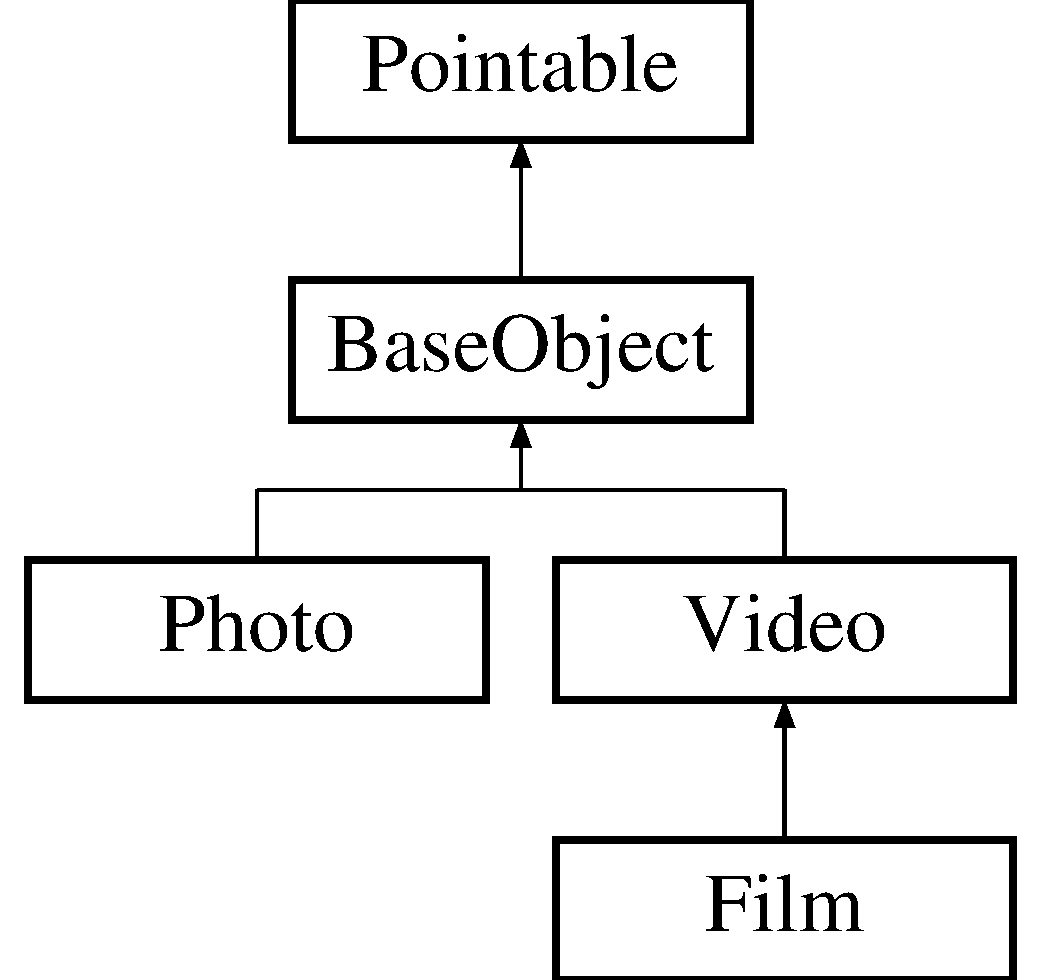
\includegraphics[height=3.000000cm]{classBaseObject}
\end{center}
\end{figure}
\subsection*{Public Member Functions}
\begin{DoxyCompactItemize}
\item 
\hypertarget{classBaseObject_ac9e64a371856dc974183c1b04bfdd0c9}{\hyperlink{classBaseObject_ac9e64a371856dc974183c1b04bfdd0c9}{Base\-Object} ()}\label{classBaseObject_ac9e64a371856dc974183c1b04bfdd0c9}

\begin{DoxyCompactList}\small\item\em Parameterless Constructor. \end{DoxyCompactList}\item 
\hypertarget{classBaseObject_aef7d506580d526367abe614c614aaf43}{\hyperlink{classBaseObject_aef7d506580d526367abe614c614aaf43}{Base\-Object} (std\-::string, time\-\_\-t, std\-::string)}\label{classBaseObject_aef7d506580d526367abe614c614aaf43}

\begin{DoxyCompactList}\small\item\em Parametered Constructor. \end{DoxyCompactList}\item 
virtual \hyperlink{classBaseObject_a83eecfd3bdaffda4e6c7d0fb98747f96}{$\sim$\-Base\-Object} ()
\begin{DoxyCompactList}\small\item\em Parameterless Destructor. \end{DoxyCompactList}\item 
\hypertarget{classBaseObject_a813ed6b0e98919c44c5ddf95495bfa2d}{std\-::string \hyperlink{classBaseObject_a813ed6b0e98919c44c5ddf95495bfa2d}{get\-Name} () const }\label{classBaseObject_a813ed6b0e98919c44c5ddf95495bfa2d}

\begin{DoxyCompactList}\small\item\em Returns name of multimedia object (track name, movie title etc) \end{DoxyCompactList}\item 
\hypertarget{classBaseObject_a1d9abdd27cea258333a27d505c57e857}{time\-\_\-t \hyperlink{classBaseObject_a1d9abdd27cea258333a27d505c57e857}{get\-Creation\-Date} () const }\label{classBaseObject_a1d9abdd27cea258333a27d505c57e857}

\begin{DoxyCompactList}\small\item\em Returns date of creation as time\-\_\-t. \end{DoxyCompactList}\item 
\hypertarget{classBaseObject_a46ce6977e2a06f0785aca14454df9d94}{std\-::string \hyperlink{classBaseObject_a46ce6977e2a06f0785aca14454df9d94}{get\-Path} () const }\label{classBaseObject_a46ce6977e2a06f0785aca14454df9d94}

\begin{DoxyCompactList}\small\item\em Returns unix path (including filename) of object. \end{DoxyCompactList}\item 
\hypertarget{classBaseObject_a3999488d0dd4e825641ece8f332385e1}{void \hyperlink{classBaseObject_a3999488d0dd4e825641ece8f332385e1}{set\-Name} (std\-::string)}\label{classBaseObject_a3999488d0dd4e825641ece8f332385e1}

\begin{DoxyCompactList}\small\item\em Sets name of multimedia object (track name, movie title etc) \end{DoxyCompactList}\item 
\hypertarget{classBaseObject_aeeb327051d61bd727722f583fa0bc41c}{void \hyperlink{classBaseObject_aeeb327051d61bd727722f583fa0bc41c}{set\-Creation\-Date} (time\-\_\-t)}\label{classBaseObject_aeeb327051d61bd727722f583fa0bc41c}

\begin{DoxyCompactList}\small\item\em Sets date of creation as time\-\_\-t. \end{DoxyCompactList}\item 
\hypertarget{classBaseObject_a06461859fe33fc77fee0b74dbbe1b57d}{void \hyperlink{classBaseObject_a06461859fe33fc77fee0b74dbbe1b57d}{set\-Path} (std\-::string)}\label{classBaseObject_a06461859fe33fc77fee0b74dbbe1b57d}

\begin{DoxyCompactList}\small\item\em Sets unix path (including filename) of object. \end{DoxyCompactList}\item 
\hypertarget{classBaseObject_aab08eee6684fdfa0852b1f914379b9c4}{virtual std\-::string \hyperlink{classBaseObject_aab08eee6684fdfa0852b1f914379b9c4}{to\-String} () const }\label{classBaseObject_aab08eee6684fdfa0852b1f914379b9c4}

\begin{DoxyCompactList}\small\item\em Returns multi-\/line string containing formatted description of object. \end{DoxyCompactList}\item 
void \hyperlink{classBaseObject_a9bad65dddde7dec1ea622edce664cc9f}{print} () const 
\begin{DoxyCompactList}\small\item\em Prints formatted description of object. \end{DoxyCompactList}\end{DoxyCompactItemize}


\subsection{Detailed Description}
Base multimedia-\/type file object. 

This class is the base class for all objects which describe multimedia files in the project. 

\subsection{Constructor \& Destructor Documentation}
\hypertarget{classBaseObject_a83eecfd3bdaffda4e6c7d0fb98747f96}{\index{Base\-Object@{Base\-Object}!$\sim$\-Base\-Object@{$\sim$\-Base\-Object}}
\index{$\sim$\-Base\-Object@{$\sim$\-Base\-Object}!BaseObject@{Base\-Object}}
\subsubsection[{$\sim$\-Base\-Object}]{\setlength{\rightskip}{0pt plus 5cm}Base\-Object\-::$\sim$\-Base\-Object (
\begin{DoxyParamCaption}
{}
\end{DoxyParamCaption}
)\hspace{0.3cm}{\ttfamily [virtual]}}}\label{classBaseObject_a83eecfd3bdaffda4e6c7d0fb98747f96}


Parameterless Destructor. 

Implemetation is empty as there is nothing to delete. 

\subsection{Member Function Documentation}
\hypertarget{classBaseObject_a9bad65dddde7dec1ea622edce664cc9f}{\index{Base\-Object@{Base\-Object}!print@{print}}
\index{print@{print}!BaseObject@{Base\-Object}}
\subsubsection[{print}]{\setlength{\rightskip}{0pt plus 5cm}void Base\-Object\-::print (
\begin{DoxyParamCaption}
{}
\end{DoxyParamCaption}
) const}}\label{classBaseObject_a9bad65dddde7dec1ea622edce664cc9f}


Prints formatted description of object. 

This function prints out a description of the object, usually by displaying the values of each member variable. It does this by calling the \hyperlink{classBaseObject_aab08eee6684fdfa0852b1f914379b9c4}{to\-String()} function of the object. Thus that function is virtual, so that subclasses of \hyperlink{classBaseObject}{Base\-Object} can effectively reimplement this function to include extra member data. 

The documentation for this class was generated from the following files\-:\begin{DoxyCompactItemize}
\item 
Base\-Object.\-h\item 
Base\-Object.\-cpp\end{DoxyCompactItemize}

\hypertarget{classFilm}{\section{Film Class Reference}
\label{classFilm}\index{Film@{Film}}
}


\hyperlink{classFilm}{Film} file object.  




{\ttfamily \#include $<$Film.\-h$>$}

Inheritance diagram for Film\-:\begin{figure}[H]
\begin{center}
\leavevmode
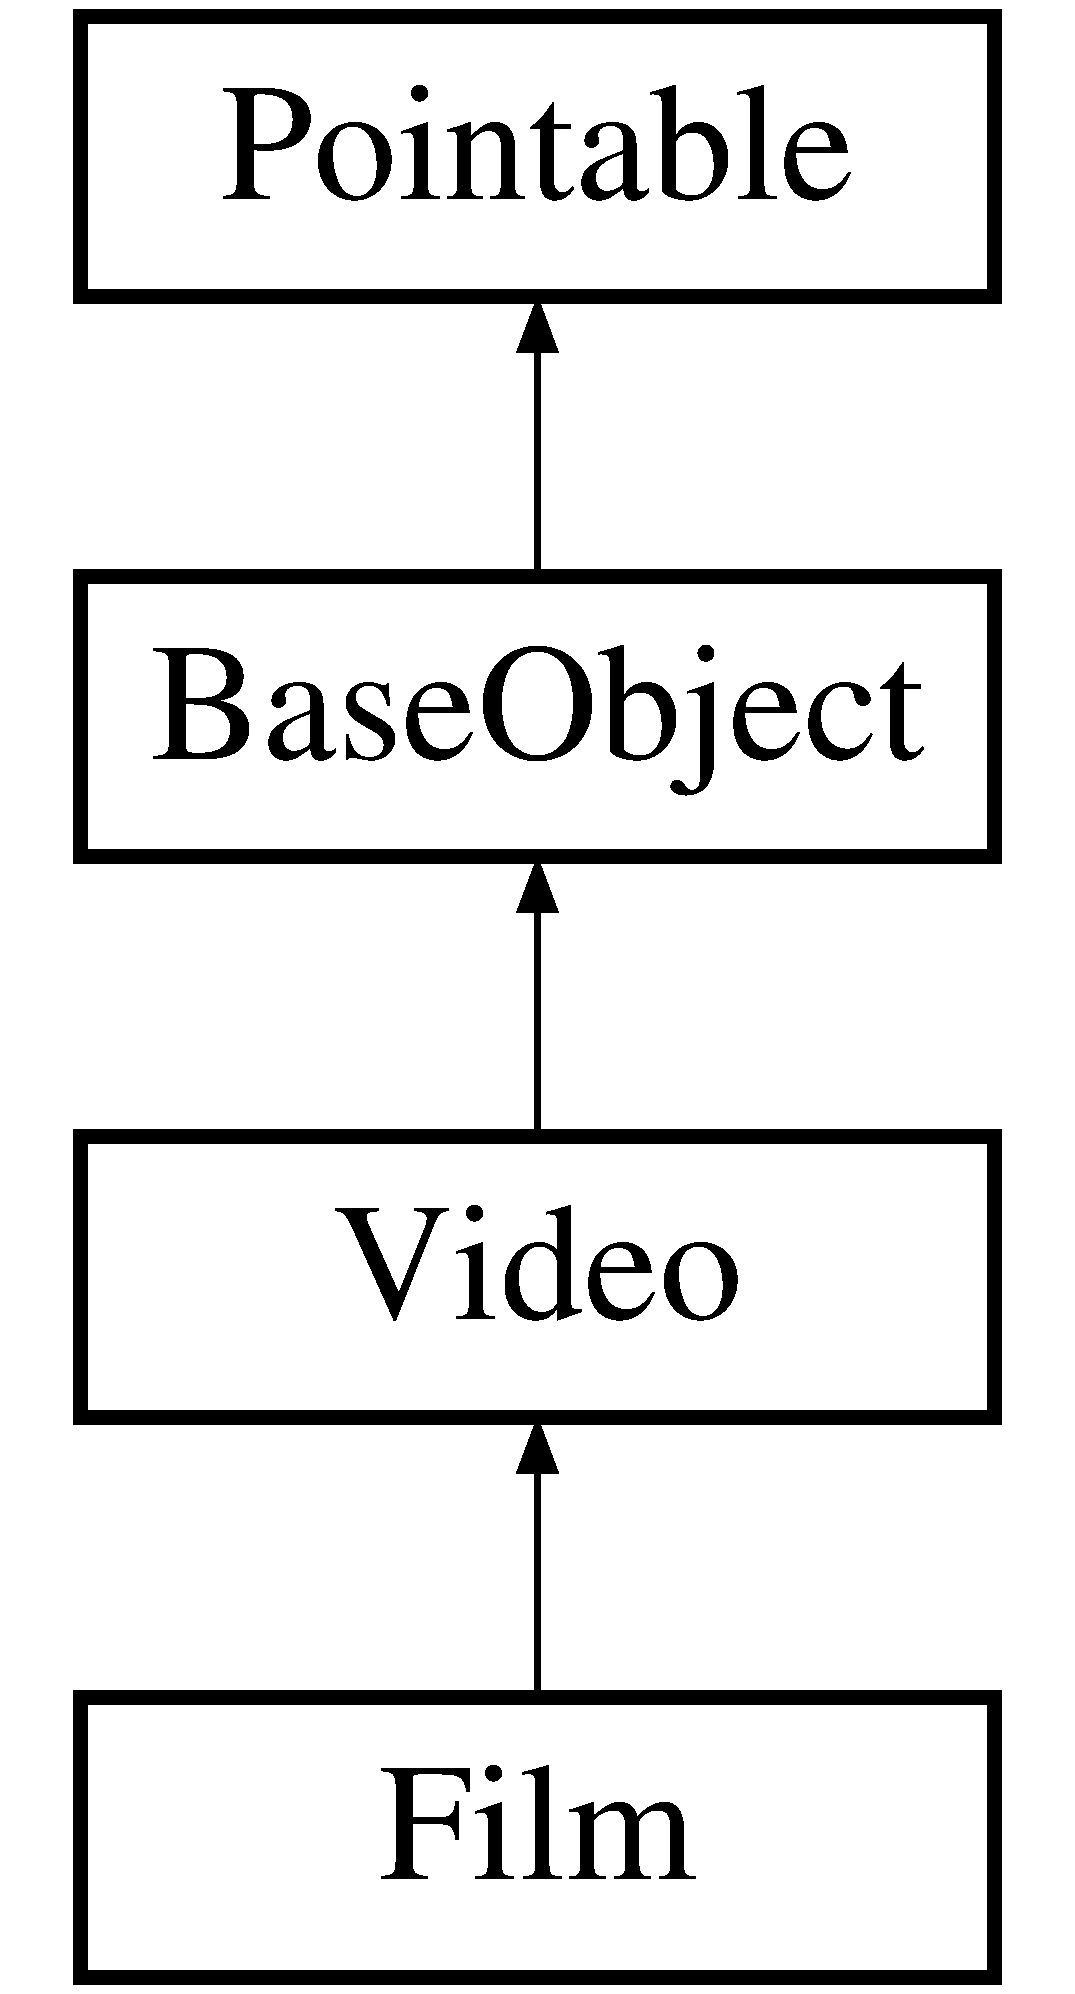
\includegraphics[height=4.000000cm]{classFilm}
\end{center}
\end{figure}
\subsection*{Public Member Functions}
\begin{DoxyCompactItemize}
\item 
\hypertarget{classFilm_a704092a2bb7629c5bf053c8011e148ee}{\hyperlink{classFilm_a704092a2bb7629c5bf053c8011e148ee}{Film} (const std\-::string \&name=\char`\"{}new film\char`\"{}, time\-\_\-t creat=time(N\-U\-L\-L), const std\-::string \&path=\char`\"{}$\sim$/new\-\_\-film\char`\"{}, int duration=0, int chapter\-\_\-count=0, int $\ast$chapters=N\-U\-L\-L)}\label{classFilm_a704092a2bb7629c5bf053c8011e148ee}

\begin{DoxyCompactList}\small\item\em Parametered Constructor. \end{DoxyCompactList}\item 
\hypertarget{classFilm_a34c9de2efb9554ce1192e4110d98806b}{\hyperlink{classFilm_a34c9de2efb9554ce1192e4110d98806b}{Film} (const \hyperlink{classFilm}{Film} \&)}\label{classFilm_a34c9de2efb9554ce1192e4110d98806b}

\begin{DoxyCompactList}\small\item\em Copy Constructor. \end{DoxyCompactList}\item 
virtual \hyperlink{classFilm_a8dab653f8a6c0635ca5ddbe0bbdd9a25}{$\sim$\-Film} ()
\begin{DoxyCompactList}\small\item\em Parameterless Destructor. \end{DoxyCompactList}\item 
\hypertarget{classFilm_a413b52608cd8103e74d3ee7ea8026e17}{virtual std\-::string \hyperlink{classFilm_a413b52608cd8103e74d3ee7ea8026e17}{to\-String} (bool=false) const }\label{classFilm_a413b52608cd8103e74d3ee7ea8026e17}

\begin{DoxyCompactList}\small\item\em Returns multi-\/line string containing formatted description of object. \end{DoxyCompactList}\item 
\hypertarget{classFilm_ab0c2831b76a6b932dfc4a6facc38870c}{void \hyperlink{classFilm_ab0c2831b76a6b932dfc4a6facc38870c}{set\-Chapters} (const int $\ast$, int)}\label{classFilm_ab0c2831b76a6b932dfc4a6facc38870c}

\begin{DoxyCompactList}\small\item\em setter for chapters array. must also pass length of array, which sets Chapter\-Count \end{DoxyCompactList}\item 
\hypertarget{classFilm_ad0fa928009af1be1c176d06d55c14e11}{const int $\ast$ \hyperlink{classFilm_ad0fa928009af1be1c176d06d55c14e11}{get\-Chapters} (void) const }\label{classFilm_ad0fa928009af1be1c176d06d55c14e11}

\begin{DoxyCompactList}\small\item\em getter for chapter array \end{DoxyCompactList}\item 
\hypertarget{classFilm_a3e07b723255ff357d3f459b08c5fa39e}{int \hyperlink{classFilm_a3e07b723255ff357d3f459b08c5fa39e}{get\-Chapter\-Count} (void) const }\label{classFilm_a3e07b723255ff357d3f459b08c5fa39e}

\begin{DoxyCompactList}\small\item\em getter for number of chapters \end{DoxyCompactList}\end{DoxyCompactItemize}


\subsection{Detailed Description}
\hyperlink{classFilm}{Film} file object. 

This class describes a \hyperlink{classFilm}{Film} object 

\subsection{Constructor \& Destructor Documentation}
\hypertarget{classFilm_a8dab653f8a6c0635ca5ddbe0bbdd9a25}{\index{Film@{Film}!$\sim$\-Film@{$\sim$\-Film}}
\index{$\sim$\-Film@{$\sim$\-Film}!Film@{Film}}
\subsubsection[{$\sim$\-Film}]{\setlength{\rightskip}{0pt plus 5cm}Film\-::$\sim$\-Film (
\begin{DoxyParamCaption}
{}
\end{DoxyParamCaption}
)\hspace{0.3cm}{\ttfamily [virtual]}}}\label{classFilm_a8dab653f8a6c0635ca5ddbe0bbdd9a25}


Parameterless Destructor. 

Deletes table of chapters. 

The documentation for this class was generated from the following files\-:\begin{DoxyCompactItemize}
\item 
Film.\-h\item 
Film.\-cpp\end{DoxyCompactItemize}

\hypertarget{classGroup}{\section{Group Class Reference}
\label{classGroup}\index{Group@{Group}}
}


Container Class for Multimedia Objects.  




{\ttfamily \#include $<$Group.\+h$>$}

Inheritance diagram for Group\+:\begin{figure}[H]
\begin{center}
\leavevmode
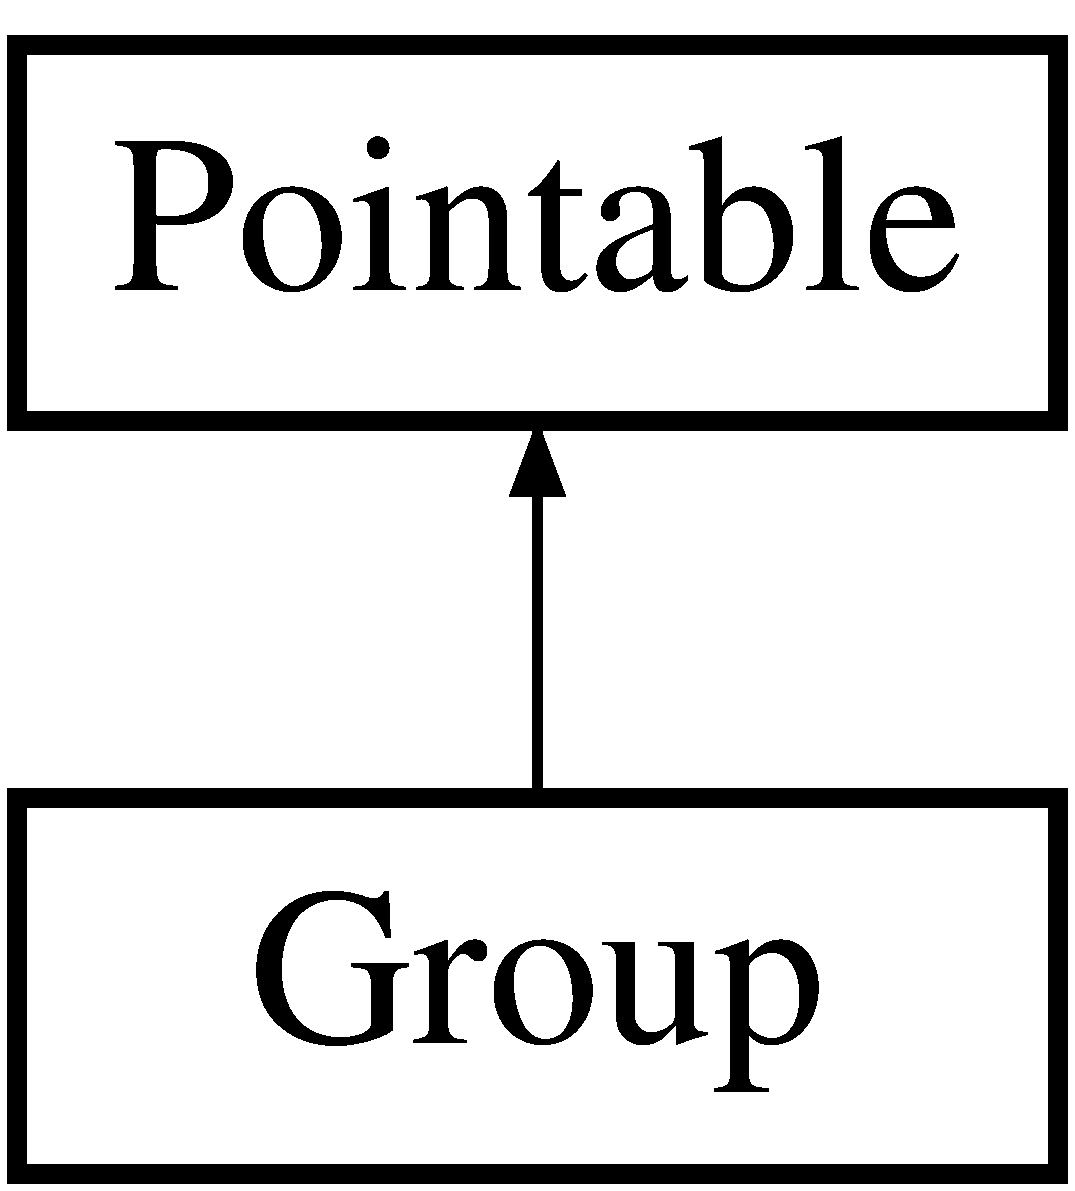
\includegraphics[height=2.000000cm]{classGroup}
\end{center}
\end{figure}
\subsection*{Public Member Functions}
\begin{DoxyCompactItemize}
\item 
\hypertarget{classGroup_a7b74f9ac68e0504ccf2e2854b7355ff1}{\hyperlink{classGroup_a7b74f9ac68e0504ccf2e2854b7355ff1}{Group} ()}\label{classGroup_a7b74f9ac68e0504ccf2e2854b7355ff1}

\begin{DoxyCompactList}\small\item\em Parameterless Constructor. \end{DoxyCompactList}\item 
\hypertarget{classGroup_a03b66550c572b981322a646a129392ae}{\hyperlink{classGroup_a03b66550c572b981322a646a129392ae}{Group} (const std\+::string \&)}\label{classGroup_a03b66550c572b981322a646a129392ae}

\begin{DoxyCompactList}\small\item\em Parametered Constructor. \end{DoxyCompactList}\item 
\hypertarget{classGroup_a41e1c4f5094ed0d15e5b387a4a5349d0}{const std\+::string \& {\bfseries get\+Name} () const }\label{classGroup_a41e1c4f5094ed0d15e5b387a4a5349d0}

\item 
\hypertarget{classGroup_a70432bd4aca1a8ee19c3b104d54c0c64}{void {\bfseries print} () const }\label{classGroup_a70432bd4aca1a8ee19c3b104d54c0c64}

\item 
\hypertarget{classGroup_aad096e2bceeedd1e1ea22dac8ee614da}{std\+::string {\bfseries to\+String} () const }\label{classGroup_aad096e2bceeedd1e1ea22dac8ee614da}

\item 
\hypertarget{classGroup_aa08edc49e142c99a69f4408cf6d09785}{void {\bfseries play} () const }\label{classGroup_aa08edc49e142c99a69f4408cf6d09785}

\end{DoxyCompactItemize}


\subsection{Detailed Description}
Container Class for Multimedia Objects. 

This class gives a way to assign Multimedia Objects to a group. 

The documentation for this class was generated from the following files\+:\begin{DoxyCompactItemize}
\item 
Group.\+h\item 
Group.\+cpp\end{DoxyCompactItemize}

\hypertarget{classintrusive__ptr}{\section{intrusive\-\_\-ptr$<$ T $>$ Class Template Reference}
\label{classintrusive__ptr}\index{intrusive\-\_\-ptr$<$ T $>$@{intrusive\-\_\-ptr$<$ T $>$}}
}


{\ttfamily \#include $<$intrusive\-\_\-ptr.\-h$>$}

\subsection*{Public Types}
\begin{DoxyCompactItemize}
\item 
\hypertarget{classintrusive__ptr_ae15c9aa35038587012d1b08729cc19c9}{typedef T {\bfseries element\-\_\-type}}\label{classintrusive__ptr_ae15c9aa35038587012d1b08729cc19c9}

\end{DoxyCompactItemize}
\subsection*{Public Member Functions}
\begin{DoxyCompactItemize}
\item 
\hypertarget{classintrusive__ptr_a1a462a7c6f3247828d8360ca04511237}{{\bfseries intrusive\-\_\-ptr} (T $\ast$p, bool add\-\_\-ref=true)}\label{classintrusive__ptr_a1a462a7c6f3247828d8360ca04511237}

\item 
\hypertarget{classintrusive__ptr_a60d33e3607b90c2d7f315d2d0be19735}{{\footnotesize template$<$class U $>$ }\\{\bfseries intrusive\-\_\-ptr} (\hyperlink{classintrusive__ptr}{intrusive\-\_\-ptr}$<$ U $>$ const \&rhs)}\label{classintrusive__ptr_a60d33e3607b90c2d7f315d2d0be19735}

\item 
\hypertarget{classintrusive__ptr_a1a05008b03d6cfb92dfa60515cd848d8}{{\bfseries intrusive\-\_\-ptr} (\hyperlink{classintrusive__ptr}{intrusive\-\_\-ptr} const \&rhs)}\label{classintrusive__ptr_a1a05008b03d6cfb92dfa60515cd848d8}

\item 
\hypertarget{classintrusive__ptr_a3f784a56085dd6e9f711e57a803dd1dc}{{\footnotesize template$<$class U $>$ }\\\hyperlink{classintrusive__ptr}{intrusive\-\_\-ptr} \& {\bfseries operator=} (\hyperlink{classintrusive__ptr}{intrusive\-\_\-ptr}$<$ U $>$ const \&rhs)}\label{classintrusive__ptr_a3f784a56085dd6e9f711e57a803dd1dc}

\item 
\hypertarget{classintrusive__ptr_ae1f058e2b20ea4ef7c3c4c30c8c37694}{\hyperlink{classintrusive__ptr}{intrusive\-\_\-ptr} \& {\bfseries operator=} (\hyperlink{classintrusive__ptr}{intrusive\-\_\-ptr} const \&rhs)}\label{classintrusive__ptr_ae1f058e2b20ea4ef7c3c4c30c8c37694}

\item 
\hypertarget{classintrusive__ptr_acbf9dbecf8e789db853832d84e2c7e19}{\hyperlink{classintrusive__ptr}{intrusive\-\_\-ptr} \& {\bfseries operator=} (T $\ast$rhs)}\label{classintrusive__ptr_acbf9dbecf8e789db853832d84e2c7e19}

\item 
\hypertarget{classintrusive__ptr_ae360b0fffd335b683b350c154922c6db}{void {\bfseries reset} ()}\label{classintrusive__ptr_ae360b0fffd335b683b350c154922c6db}

\item 
\hypertarget{classintrusive__ptr_a81e2fb688afba02de9ecf2006caeb62e}{void {\bfseries reset} (T $\ast$rhs)}\label{classintrusive__ptr_a81e2fb688afba02de9ecf2006caeb62e}

\item 
\hypertarget{classintrusive__ptr_a70192c07e3ff5035942095a5d2d97c34}{T $\ast$ {\bfseries get} () const }\label{classintrusive__ptr_a70192c07e3ff5035942095a5d2d97c34}

\item 
\hypertarget{classintrusive__ptr_a63f7f0b02c547127f9f68ecdb01f7aa6}{T \& {\bfseries operator$\ast$} () const }\label{classintrusive__ptr_a63f7f0b02c547127f9f68ecdb01f7aa6}

\item 
\hypertarget{classintrusive__ptr_a4756c9e89a1a057e2c911d8224197d31}{T $\ast$ {\bfseries operator-\/$>$} () const }\label{classintrusive__ptr_a4756c9e89a1a057e2c911d8224197d31}

\item 
\hypertarget{classintrusive__ptr_a1a71711829594617e226fada9b7ef351}{{\bfseries operator unspecified\-\_\-bool\-\_\-type} () const }\label{classintrusive__ptr_a1a71711829594617e226fada9b7ef351}

\item 
\hypertarget{classintrusive__ptr_aee167762c6829dac96f664b4ab505e39}{bool {\bfseries operator!} () const }\label{classintrusive__ptr_aee167762c6829dac96f664b4ab505e39}

\item 
\hypertarget{classintrusive__ptr_a95826a79f706bc5c6b9fd28ae334e974}{void {\bfseries swap} (\hyperlink{classintrusive__ptr}{intrusive\-\_\-ptr} \&rhs)}\label{classintrusive__ptr_a95826a79f706bc5c6b9fd28ae334e974}

\end{DoxyCompactItemize}


\subsection{Detailed Description}
\subsubsection*{template$<$class T$>$class intrusive\-\_\-ptr$<$ T $>$}

\hyperlink{classintrusive__ptr}{intrusive\-\_\-ptr}\-: a smart pointer that uses intrusive reference counting. Relies on unqualified calls to 
\begin{DoxyPre}
     void intrusive\_ptr\_add\_ref(T * p);
     void intrusive\_ptr\_release(T * p);
\end{DoxyPre}
 (p != 0)

The object is responsible for destroying itself. 

The documentation for this class was generated from the following file\-:\begin{DoxyCompactItemize}
\item 
intrusive\-\_\-ptr.\-h\end{DoxyCompactItemize}

\hypertarget{classMultFS}{\section{Mult\-F\-S Class Reference}
\label{classMultFS}\index{Mult\-F\-S@{Mult\-F\-S}}
}


Top-\/\-Level Class for Multimedia Objects.  




{\ttfamily \#include $<$Mult\-F\-S.\-h$>$}

\subsection*{Public Types}
\begin{DoxyCompactItemize}
\item 
\hypertarget{classMultFS_a3862987abee233b7ea08a67abc80b245}{typedef \hyperlink{classintrusive__ptr}{intrusive\-\_\-ptr}$<$ \hyperlink{classBaseObject}{Base\-Object} $>$ \hyperlink{classMultFS_a3862987abee233b7ea08a67abc80b245}{Mult\-Obj}}\label{classMultFS_a3862987abee233b7ea08a67abc80b245}

\begin{DoxyCompactList}\small\item\em Smart pointer to \hyperlink{classBaseObject}{Base\-Object}. \end{DoxyCompactList}\item 
\hypertarget{classMultFS_a0c5fea8cc8ab29c2624d5863cf75cc6f}{typedef \hyperlink{classintrusive__ptr}{intrusive\-\_\-ptr}$<$ \hyperlink{classGroup}{Group} $>$ \hyperlink{classMultFS_a0c5fea8cc8ab29c2624d5863cf75cc6f}{Mult\-Gr}}\label{classMultFS_a0c5fea8cc8ab29c2624d5863cf75cc6f}

\begin{DoxyCompactList}\small\item\em Smart pointer to \hyperlink{classGroup}{Group}. \end{DoxyCompactList}\end{DoxyCompactItemize}
\subsection*{Public Member Functions}
\begin{DoxyCompactItemize}
\item 
\hypertarget{classMultFS_aacf6a025364bd168fbd6dd37aaa6a152}{\hyperlink{classMultFS_a3862987abee233b7ea08a67abc80b245}{Mult\-Obj} \hyperlink{classMultFS_aacf6a025364bd168fbd6dd37aaa6a152}{create} (\hyperlink{classBaseObject}{Base\-Object} $\ast$)}\label{classMultFS_aacf6a025364bd168fbd6dd37aaa6a152}

\begin{DoxyCompactList}\small\item\em Adds a new object to the object container. Depricated. \end{DoxyCompactList}\item 
\hypertarget{classMultFS_abd99f17847032c1f667843e2bd72c57c}{\hyperlink{classMultFS_a0c5fea8cc8ab29c2624d5863cf75cc6f}{Mult\-Gr} \hyperlink{classMultFS_abd99f17847032c1f667843e2bd72c57c}{create} (\hyperlink{classGroup}{Group} $\ast$)}\label{classMultFS_abd99f17847032c1f667843e2bd72c57c}

\begin{DoxyCompactList}\small\item\em Adds a new group to the groups container. Depricated. \end{DoxyCompactList}\item 
\hypertarget{classMultFS_a96e45921965aa794c03c95d046a0f1b8}{\hyperlink{classMultFS_a3862987abee233b7ea08a67abc80b245}{Mult\-Obj} {\bfseries create\-Obj} (const std\-::string \&)}\label{classMultFS_a96e45921965aa794c03c95d046a0f1b8}

\item 
\hypertarget{classMultFS_a833b6278499d1e187f3828d39b936eaf}{\hyperlink{classMultFS_a0c5fea8cc8ab29c2624d5863cf75cc6f}{Mult\-Gr} {\bfseries create\-Gr} (const std\-::string \&)}\label{classMultFS_a833b6278499d1e187f3828d39b936eaf}

\item 
\hypertarget{classMultFS_a8f223d40df0273ae8eccfc15c8925765}{void \hyperlink{classMultFS_a8f223d40df0273ae8eccfc15c8925765}{remove} (const std\-::string \&)}\label{classMultFS_a8f223d40df0273ae8eccfc15c8925765}

\begin{DoxyCompactList}\small\item\em Removes objects and groups by name. \end{DoxyCompactList}\item 
\hypertarget{classMultFS_a7cee8ae014447fb24cf1efd5a3024101}{std\-::string \hyperlink{classMultFS_a7cee8ae014447fb24cf1efd5a3024101}{search} (const std\-::string \&) const }\label{classMultFS_a7cee8ae014447fb24cf1efd5a3024101}

\begin{DoxyCompactList}\small\item\em Return a string containing details of objects and groups with the given name. \end{DoxyCompactList}\item 
\hypertarget{classMultFS_a6f9ba46bf4916e4c1534a41f9222135a}{bool \hyperlink{classMultFS_a6f9ba46bf4916e4c1534a41f9222135a}{play} (const std\-::string \&) const }\label{classMultFS_a6f9ba46bf4916e4c1534a41f9222135a}

\begin{DoxyCompactList}\small\item\em Plays objects and groups with the given name. \end{DoxyCompactList}\item 
\hypertarget{classMultFS_a8e9f409a1c1c51ccb64b65bec60c3168}{bool \hyperlink{classMultFS_a8e9f409a1c1c51ccb64b65bec60c3168}{write} (const std\-::string \&) const }\label{classMultFS_a8e9f409a1c1c51ccb64b65bec60c3168}

\begin{DoxyCompactList}\small\item\em Writes the list of objects to a file. \end{DoxyCompactList}\item 
int \hyperlink{classMultFS_a4b2f283bc6d3f77f920c38df6f618f65}{read} (const std\-::string \&)
\begin{DoxyCompactList}\small\item\em Reads in objects from a file. \end{DoxyCompactList}\end{DoxyCompactItemize}


\subsection{Detailed Description}
Top-\/\-Level Class for Multimedia Objects. 

This class contains all the objects and groups in the program, and is responsible for destroying or creating them. 

\subsection{Member Function Documentation}
\hypertarget{classMultFS_a4b2f283bc6d3f77f920c38df6f618f65}{\index{Mult\-F\-S@{Mult\-F\-S}!read@{read}}
\index{read@{read}!MultFS@{Mult\-F\-S}}
\subsubsection[{read}]{\setlength{\rightskip}{0pt plus 5cm}int Mult\-F\-S\-::read (
\begin{DoxyParamCaption}
\item[{const std\-::string \&}]{}
\end{DoxyParamCaption}
)}}\label{classMultFS_a4b2f283bc6d3f77f920c38df6f618f65}


Reads in objects from a file. 

Return value is the number of objects not read due to name conflicts 

The documentation for this class was generated from the following files\-:\begin{DoxyCompactItemize}
\item 
Mult\-F\-S.\-h\item 
Mult\-F\-S.\-cpp\end{DoxyCompactItemize}

\hypertarget{classPhoto}{\section{Photo Class Reference}
\label{classPhoto}\index{Photo@{Photo}}
}


\hyperlink{classPhoto}{Photo} file object.  




{\ttfamily \#include $<$Photo.\+h$>$}

Inheritance diagram for Photo\+:\begin{figure}[H]
\begin{center}
\leavevmode
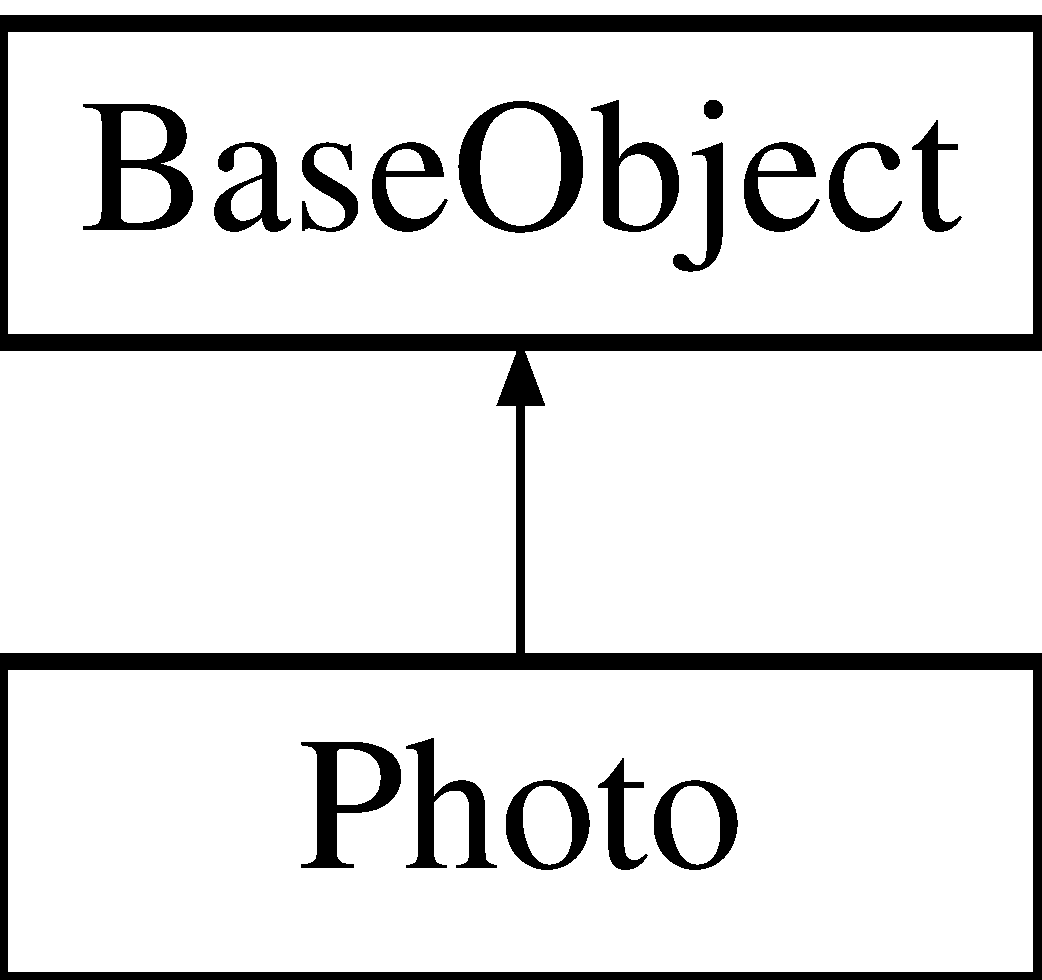
\includegraphics[height=3.000000cm]{classPhoto}
\end{center}
\end{figure}
\subsection*{Public Member Functions}
\begin{DoxyCompactItemize}
\item 
\hypertarget{classPhoto_ab07e00487a31f231f4730b3859664da5}{\hyperlink{classPhoto_ab07e00487a31f231f4730b3859664da5}{Photo} (const std\+::string \&name=\char`\"{}new photo\char`\"{}, time\+\_\+t creat=time(N\+U\+L\+L), const std\+::string \&path=\char`\"{}$\sim$/new\+\_\+photo\char`\"{}, const std\+::string \&place=\char`\"{}\char`\"{})}\label{classPhoto_ab07e00487a31f231f4730b3859664da5}

\begin{DoxyCompactList}\small\item\em Parametered Constructor. \end{DoxyCompactList}\item 
virtual \hyperlink{classPhoto_adc366234be6226600360c7cbba8e7fcf}{$\sim$\+Photo} ()
\begin{DoxyCompactList}\small\item\em Parameterless Destructor. \end{DoxyCompactList}\item 
\hypertarget{classPhoto_a8be4be2bb68b6db13ec45ff3bed71481}{virtual std\+::string \hyperlink{classPhoto_a8be4be2bb68b6db13ec45ff3bed71481}{to\+String} (void) const }\label{classPhoto_a8be4be2bb68b6db13ec45ff3bed71481}

\begin{DoxyCompactList}\small\item\em Returns multi-\/line string containing formatted description of object. \end{DoxyCompactList}\item 
\hypertarget{classPhoto_a145e0540284cbc678ef5bdb02a8fcaa8}{virtual void \hyperlink{classPhoto_a145e0540284cbc678ef5bdb02a8fcaa8}{play} ()}\label{classPhoto_a145e0540284cbc678ef5bdb02a8fcaa8}

\begin{DoxyCompactList}\small\item\em Opens file in external player. \end{DoxyCompactList}\item 
\hypertarget{classPhoto_a310123a0d107ab078bc83a80b484e2c1}{const std\+::string \& \hyperlink{classPhoto_a310123a0d107ab078bc83a80b484e2c1}{get\+Place} (void) const }\label{classPhoto_a310123a0d107ab078bc83a80b484e2c1}

\begin{DoxyCompactList}\small\item\em getter for place \end{DoxyCompactList}\item 
\hypertarget{classPhoto_ae835a7d23db2b2f6b90d1efaaf034959}{void \hyperlink{classPhoto_ae835a7d23db2b2f6b90d1efaaf034959}{set\+Place} (const std\+::string \&)}\label{classPhoto_ae835a7d23db2b2f6b90d1efaaf034959}

\begin{DoxyCompactList}\small\item\em setter for place \end{DoxyCompactList}\end{DoxyCompactItemize}


\subsection{Detailed Description}
\hyperlink{classPhoto}{Photo} file object. 

This class describes a \hyperlink{classPhoto}{Photo} object 

\subsection{Constructor \& Destructor Documentation}
\hypertarget{classPhoto_adc366234be6226600360c7cbba8e7fcf}{\index{Photo@{Photo}!````~Photo@{$\sim$\+Photo}}
\index{````~Photo@{$\sim$\+Photo}!Photo@{Photo}}
\subsubsection[{$\sim$\+Photo}]{\setlength{\rightskip}{0pt plus 5cm}Photo\+::$\sim$\+Photo (
\begin{DoxyParamCaption}
{}
\end{DoxyParamCaption}
)\hspace{0.3cm}{\ttfamily [virtual]}}}\label{classPhoto_adc366234be6226600360c7cbba8e7fcf}


Parameterless Destructor. 

Implemetation is empty as there is nothing to delete. 

The documentation for this class was generated from the following files\+:\begin{DoxyCompactItemize}
\item 
Photo.\+h\item 
Photo.\+cpp\end{DoxyCompactItemize}

\hypertarget{classPointable}{\section{Pointable Class Reference}
\label{classPointable}\index{Pointable@{Pointable}}
}


{\ttfamily \#include $<$intrusive\-\_\-ptr.\-h$>$}

Inheritance diagram for Pointable\-:\begin{figure}[H]
\begin{center}
\leavevmode
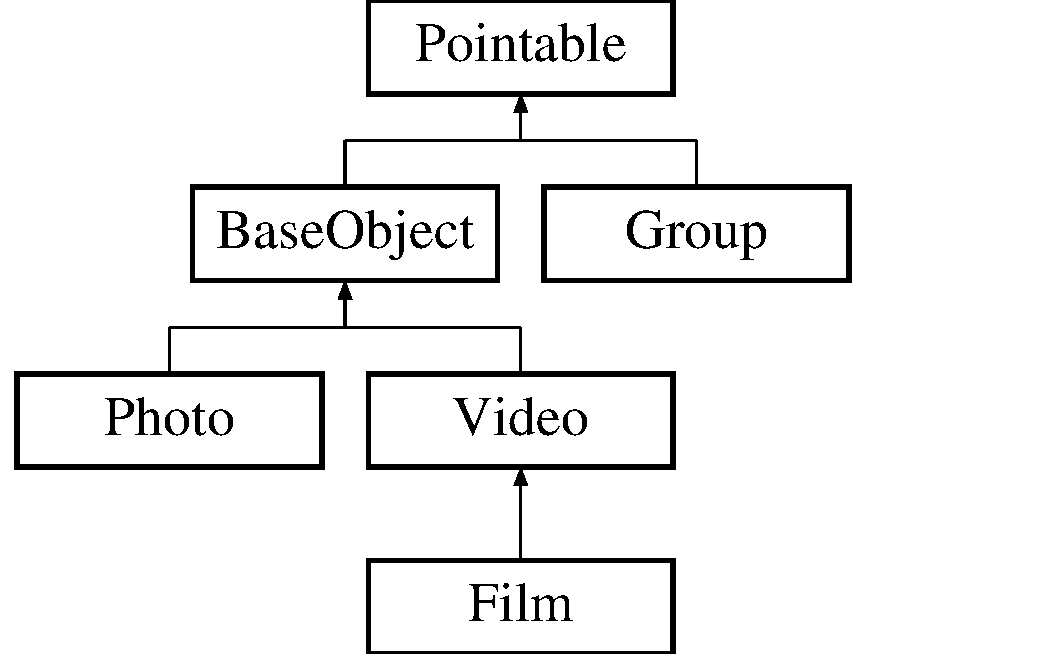
\includegraphics[height=4.000000cm]{classPointable}
\end{center}
\end{figure}
\subsection*{Public Member Functions}
\begin{DoxyCompactItemize}
\item 
\hypertarget{classPointable_adc4da364054bdd4c4a9624f5dc190c8a}{{\bfseries Pointable} (const \hyperlink{classPointable}{Pointable} \&)}\label{classPointable_adc4da364054bdd4c4a9624f5dc190c8a}

\item 
\hypertarget{classPointable_a8a7eb6956905e6e320ce97fa24f03b59}{\hyperlink{classPointable}{Pointable} \& {\bfseries operator=} (const \hyperlink{classPointable}{Pointable} \&)}\label{classPointable_a8a7eb6956905e6e320ce97fa24f03b59}

\end{DoxyCompactItemize}
\subsection*{Friends}
\begin{DoxyCompactItemize}
\item 
\hypertarget{classPointable_a9c08ce04af1d8cd2697b64990c51a5f4}{long {\bfseries intrusive\-\_\-ptr\-\_\-get\-\_\-count} (\hyperlink{classPointable}{Pointable} $\ast$p)}\label{classPointable_a9c08ce04af1d8cd2697b64990c51a5f4}

\item 
\hypertarget{classPointable_a16ec5f964af06a93d6c7cfe0979ff672}{void {\bfseries intrusive\-\_\-ptr\-\_\-add\-\_\-ref} (\hyperlink{classPointable}{Pointable} $\ast$p)}\label{classPointable_a16ec5f964af06a93d6c7cfe0979ff672}

\item 
\hypertarget{classPointable_aee25e5a73726af47eb078e2087eaee57}{void {\bfseries intrusive\-\_\-ptr\-\_\-release} (\hyperlink{classPointable}{Pointable} $\ast$p)}\label{classPointable_aee25e5a73726af47eb078e2087eaee57}

\end{DoxyCompactItemize}


\subsection{Detailed Description}
Generic base class for objects that can be pointed by an \hyperlink{classintrusive__ptr}{intrusive\-\_\-ptr}.
\begin{DoxyItemize}
\item \begin{DoxySeeAlso}{See Also}
\hyperlink{classintrusive__ptr}{intrusive\-\_\-ptr} for details
\end{DoxySeeAlso}

\item misc. checkings are performed if macro S\-M\-A\-R\-T\-\_\-\-P\-T\-R\-\_\-\-D\-E\-B\-U\-G is defined before including \hyperlink{intrusive__ptr_8h_source}{intrusive\-\_\-ptr.\-h}
\item debug messages are displayed on stderr if macros S\-M\-A\-R\-T\-\_\-\-P\-T\-R\-\_\-\-D\-E\-B\-U\-G and if S\-M\-A\-R\-T\-\_\-\-P\-T\-R\-\_\-\-D\-E\-B\-U\-G\-\_\-\-M\-E\-S\-S\-A\-G\-E\-S are both defined. 
\end{DoxyItemize}

The documentation for this class was generated from the following file\-:\begin{DoxyCompactItemize}
\item 
intrusive\-\_\-ptr.\-h\end{DoxyCompactItemize}

\hypertarget{classServerSocket}{\section{Server\+Socket Class Reference}
\label{classServerSocket}\index{Server\+Socket@{Server\+Socket}}
}


{\ttfamily \#include $<$Socket.\+h$>$}

\subsection*{Public Member Functions}
\begin{DoxyCompactItemize}
\item 
\hyperlink{classServerSocket_a2b3098589541243241ca25495155186c}{Server\+Socket} ()
\item 
virtual \hyperlink{classSocket}{Socket} $\ast$ \hyperlink{classServerSocket_accc3d56d42aa50a5f3c920cf0b26959b}{accept} ()
\item 
virtual int \hyperlink{classServerSocket_ad5281fe6c005bca007a9a758bd612481}{bind} (int port, int backlog=50)
\item 
\hypertarget{classServerSocket_a3eac6d5571bb092622d328dbda2de2cf}{virtual int \hyperlink{classServerSocket_a3eac6d5571bb092622d328dbda2de2cf}{close} ()}\label{classServerSocket_a3eac6d5571bb092622d328dbda2de2cf}

\begin{DoxyCompactList}\small\item\em Closes the socket. \end{DoxyCompactList}\item 
\hypertarget{classServerSocket_a73a32b4697d3ff2bc9a68700f06e4dfb}{int \hyperlink{classServerSocket_a73a32b4697d3ff2bc9a68700f06e4dfb}{get\+File\+Descriptor} () const }\label{classServerSocket_a73a32b4697d3ff2bc9a68700f06e4dfb}

\begin{DoxyCompactList}\small\item\em Returns the file descriptor of the socket. \end{DoxyCompactList}\item 
void \hyperlink{classServerSocket_afe81d7c30d1e963e6a043b868560dbbd}{handle\+Sig\+Pipe} (void($\ast$function)(int signal))
\item 
void \hyperlink{classServerSocket_ac159a12414df54dfef149a8de6aacb20}{ignore\+Sig\+Pipe} ()
\begin{DoxyCompactList}\small\item\em Ignore S\+I\+G\+P\+I\+P\+E signals (. \end{DoxyCompactList}\item 
int \hyperlink{classServerSocket_a7ad8a5581c52046e641b32d96eb23406}{get\+Option} (int level, int optname, void $\ast$optval, socklen\+\_\+t $\ast$optlen)
\item 
int \hyperlink{classServerSocket_ad69fa5c5891f028192a291044b9191e2}{set\+Option} (int level, int optname, const void $\ast$optval, socklen\+\_\+t optlen)
\item 
\hypertarget{classServerSocket_ab34154bc6114c638ae02f5e018121099}{int \hyperlink{classServerSocket_ab34154bc6114c638ae02f5e018121099}{set\+Receive\+Buffer\+Size} (int size)}\label{classServerSocket_ab34154bc6114c638ae02f5e018121099}

\begin{DoxyCompactList}\small\item\em Sets the S\+O\+\_\+\+R\+C\+V\+B\+U\+F option to the specified value. \end{DoxyCompactList}\item 
\hypertarget{classServerSocket_ae60d7cc31ad535e5d3cac42e38b8ec98}{int \hyperlink{classServerSocket_ae60d7cc31ad535e5d3cac42e38b8ec98}{set\+Reuse\+Address} (bool)}\label{classServerSocket_ae60d7cc31ad535e5d3cac42e38b8ec98}

\begin{DoxyCompactList}\small\item\em Enables/disables the S\+O\+\_\+\+R\+E\+U\+S\+E\+A\+D\+D\+R socket option. \end{DoxyCompactList}\item 
\hypertarget{classServerSocket_aedb9144c9c375fcb14ac47bcb9d2eb17}{int \hyperlink{classServerSocket_aedb9144c9c375fcb14ac47bcb9d2eb17}{set\+So\+Timeout} (int timeout)}\label{classServerSocket_aedb9144c9c375fcb14ac47bcb9d2eb17}

\begin{DoxyCompactList}\small\item\em Enables/disables S\+O\+\_\+\+T\+I\+M\+E\+O\+U\+T with the specified timeout (in milliseconds). \end{DoxyCompactList}\item 
\hypertarget{classServerSocket_a9e5e1ee852ba26156c757a0086b780fe}{int \hyperlink{classServerSocket_a9e5e1ee852ba26156c757a0086b780fe}{set\+Tcp\+No\+Delay} (bool)}\label{classServerSocket_a9e5e1ee852ba26156c757a0086b780fe}

\begin{DoxyCompactList}\small\item\em Turns on/off T\+C\+P coalescence (useful in some cases to avoid delays). \end{DoxyCompactList}\end{DoxyCompactItemize}


\subsection{Detailed Description}
T\+C\+P/\+I\+P \hyperlink{classSocket}{Socket} Server. Note\+: this class supports A\+F\+\_\+\+I\+N\+E\+T connections following the I\+Pv4 Internet protocol. Other families, such as A\+F\+\_\+\+I\+N\+E\+T6 or A\+F\+\_\+\+U\+N\+I\+X are not yet supported. 

\subsection{Constructor \& Destructor Documentation}
\hypertarget{classServerSocket_a2b3098589541243241ca25495155186c}{\index{Server\+Socket@{Server\+Socket}!Server\+Socket@{Server\+Socket}}
\index{Server\+Socket@{Server\+Socket}!Server\+Socket@{Server\+Socket}}
\subsubsection[{Server\+Socket}]{\setlength{\rightskip}{0pt plus 5cm}Server\+Socket\+::\+Server\+Socket (
\begin{DoxyParamCaption}
{}
\end{DoxyParamCaption}
)}}\label{classServerSocket_a2b3098589541243241ca25495155186c}
creates a new \hyperlink{classServerSocket}{Server\+Socket}. Creates a listening A\+F\+\_\+\+I\+N\+E\+T socket (using the I\+Pv4 Internet protocol) that waits for connection requests by T\+C\+P/\+I\+P (S\+O\+C\+K\+\_\+\+S\+T\+R\+E\+A\+M) client sockets. 

\subsection{Member Function Documentation}
\hypertarget{classServerSocket_accc3d56d42aa50a5f3c920cf0b26959b}{\index{Server\+Socket@{Server\+Socket}!accept@{accept}}
\index{accept@{accept}!Server\+Socket@{Server\+Socket}}
\subsubsection[{accept}]{\setlength{\rightskip}{0pt plus 5cm}{\bf Socket} $\ast$ Server\+Socket\+::accept (
\begin{DoxyParamCaption}
{}
\end{DoxyParamCaption}
)\hspace{0.3cm}{\ttfamily [virtual]}}}\label{classServerSocket_accc3d56d42aa50a5f3c920cf0b26959b}
Accepts a new connection request and returns the corresponding socket. By default, this function blocks the caller until a connection is present \begin{DoxyReturn}{Returns}
Returns the new \hyperlink{classSocket}{Socket} or N\+U\+L\+L on error 
\end{DoxyReturn}
\hypertarget{classServerSocket_ad5281fe6c005bca007a9a758bd612481}{\index{Server\+Socket@{Server\+Socket}!bind@{bind}}
\index{bind@{bind}!Server\+Socket@{Server\+Socket}}
\subsubsection[{bind}]{\setlength{\rightskip}{0pt plus 5cm}int Server\+Socket\+::bind (
\begin{DoxyParamCaption}
\item[{int}]{port, }
\item[{int}]{backlog = {\ttfamily 50}}
\end{DoxyParamCaption}
)\hspace{0.3cm}{\ttfamily [virtual]}}}\label{classServerSocket_ad5281fe6c005bca007a9a758bd612481}
Assigns the socket to the local address. \begin{DoxyReturn}{Returns}
0 on success or a negative value on error which is one of \hyperlink{classSocket_a9f68308228badcdd299cd83e62e36976}{Socket\+::\+Errors} 
\end{DoxyReturn}
\hypertarget{classServerSocket_a7ad8a5581c52046e641b32d96eb23406}{\index{Server\+Socket@{Server\+Socket}!get\+Option@{get\+Option}}
\index{get\+Option@{get\+Option}!Server\+Socket@{Server\+Socket}}
\subsubsection[{get\+Option}]{\setlength{\rightskip}{0pt plus 5cm}int Server\+Socket\+::get\+Option (
\begin{DoxyParamCaption}
\item[{int}]{level, }
\item[{int}]{optname, }
\item[{void $\ast$}]{optval, }
\item[{socklen\+\_\+t $\ast$}]{optlen}
\end{DoxyParamCaption}
)}}\label{classServerSocket_a7ad8a5581c52046e641b32d96eb23406}
Gets socket options. Same arguments and effect as the getsockopt() system call. \begin{DoxyReturn}{Returns}
On success, zero is returned. On error, -\/1 is returned. 
\end{DoxyReturn}
\hypertarget{classServerSocket_afe81d7c30d1e963e6a043b868560dbbd}{\index{Server\+Socket@{Server\+Socket}!handle\+Sig\+Pipe@{handle\+Sig\+Pipe}}
\index{handle\+Sig\+Pipe@{handle\+Sig\+Pipe}!Server\+Socket@{Server\+Socket}}
\subsubsection[{handle\+Sig\+Pipe}]{\setlength{\rightskip}{0pt plus 5cm}void Server\+Socket\+::handle\+Sig\+Pipe (
\begin{DoxyParamCaption}
\item[{void($\ast$)(int signal)}]{function}
\end{DoxyParamCaption}
)}}\label{classServerSocket_afe81d7c30d1e963e6a043b868560dbbd}
Handle S\+I\+G\+P\+I\+P\+E signals. Sockets may abort programs by throwing a S\+I\+G\+P\+I\+P\+E signal. The function given as an argument will be called instead of aborting the program.  \hyperlink{classServerSocket_ac159a12414df54dfef149a8de6aacb20}{ignore\+Sig\+Pipe()} \hypertarget{classServerSocket_ac159a12414df54dfef149a8de6aacb20}{\index{Server\+Socket@{Server\+Socket}!ignore\+Sig\+Pipe@{ignore\+Sig\+Pipe}}
\index{ignore\+Sig\+Pipe@{ignore\+Sig\+Pipe}!Server\+Socket@{Server\+Socket}}
\subsubsection[{ignore\+Sig\+Pipe}]{\setlength{\rightskip}{0pt plus 5cm}void Server\+Socket\+::ignore\+Sig\+Pipe (
\begin{DoxyParamCaption}
{}
\end{DoxyParamCaption}
)}}\label{classServerSocket_ac159a12414df54dfef149a8de6aacb20}


Ignore S\+I\+G\+P\+I\+P\+E signals (. 

\begin{DoxySeeAlso}{See also}
\hyperlink{classServerSocket_afe81d7c30d1e963e6a043b868560dbbd}{handle\+Sig\+Pipe()}). 
\end{DoxySeeAlso}
\hypertarget{classServerSocket_ad69fa5c5891f028192a291044b9191e2}{\index{Server\+Socket@{Server\+Socket}!set\+Option@{set\+Option}}
\index{set\+Option@{set\+Option}!Server\+Socket@{Server\+Socket}}
\subsubsection[{set\+Option}]{\setlength{\rightskip}{0pt plus 5cm}int Server\+Socket\+::set\+Option (
\begin{DoxyParamCaption}
\item[{int}]{level, }
\item[{int}]{optname, }
\item[{const void $\ast$}]{optval, }
\item[{socklen\+\_\+t}]{optlen}
\end{DoxyParamCaption}
)}}\label{classServerSocket_ad69fa5c5891f028192a291044b9191e2}
Sets socket options. Same arguments and effect as the setsockopt() system call. \begin{DoxyReturn}{Returns}
On success, zero is returned. On error, -\/1 is returned.  helper functions \hyperlink{classServerSocket_ae60d7cc31ad535e5d3cac42e38b8ec98}{set\+Reuse\+Address()}, \hyperlink{classServerSocket_a9e5e1ee852ba26156c757a0086b780fe}{set\+Tcp\+No\+Delay()}, etc. 
\end{DoxyReturn}


The documentation for this class was generated from the following files\+:\begin{DoxyCompactItemize}
\item 
Socket.\+h\item 
Socket.\+cpp\end{DoxyCompactItemize}

\hypertarget{classSocket}{\section{Socket Class Reference}
\label{classSocket}\index{Socket@{Socket}}
}


{\ttfamily \#include $<$Socket.\-h$>$}

\subsection*{Public Types}
\begin{DoxyCompactItemize}
\item 
enum \hyperlink{classSocket_a9f68308228badcdd299cd83e62e36976}{Errors} \{ {\bfseries F\-A\-I\-L\-E\-D} =  -\/1, 
{\bfseries I\-N\-V\-A\-L\-I\-D\-\_\-\-S\-O\-C\-K\-E\-T} =  -\/2, 
{\bfseries U\-N\-K\-N\-O\-W\-N\-\_\-\-H\-O\-S\-T} =  -\/3
 \}
\end{DoxyCompactItemize}
\subsection*{Public Member Functions}
\begin{DoxyCompactItemize}
\item 
\hyperlink{classSocket_acd3cb39bc957be2f34c91b9e262e1cec}{Socket} (int type=S\-O\-C\-K\-\_\-\-S\-T\-R\-E\-A\-M)
\item 
\hypertarget{classSocket_a14170941ba1aaa3263f3e8dd3f85e24f}{\hyperlink{classSocket_a14170941ba1aaa3263f3e8dd3f85e24f}{Socket} (int type, int sockfd)}\label{classSocket_a14170941ba1aaa3263f3e8dd3f85e24f}

\begin{DoxyCompactList}\small\item\em Creates a socket object from an existing socket file descriptor. \end{DoxyCompactList}\item 
virtual \hyperlink{classSocket_aeac4eb6379a543d38ed88977d3b6630a}{$\sim$\-Socket} ()
\item 
virtual int \hyperlink{classSocket_a019fdc04fe2afd7aecd612469be32467}{bind} (int port=0)
\item 
virtual int \hyperlink{classSocket_a8f014a801fb3e61bbee00b84c06f2330}{bind} (const std\-::string \&host, int port)
\item 
virtual int \hyperlink{classSocket_aac9588a21bb2c52ff8246272cf36834a}{connect} (const std\-::string \&remote\-Host, int port)
\item 
virtual int \hyperlink{classSocket_aef06605c6725958004116983f1a2051f}{close} ()
\item 
\hypertarget{classSocket_a6b4449d6b454bdb4a3a809976a3c2e41}{int \hyperlink{classSocket_a6b4449d6b454bdb4a3a809976a3c2e41}{get\-File\-Descriptor} () const }\label{classSocket_a6b4449d6b454bdb4a3a809976a3c2e41}

\begin{DoxyCompactList}\small\item\em Returns the file descriptor of the socket. \end{DoxyCompactList}\item 
ssize\-\_\-t \hyperlink{classSocket_a9275eacdb64056a53cf4b9cf54cd2f1a}{send} (const void $\ast$buf, size\-\_\-t len, int flags=0)
\item 
ssize\-\_\-t \hyperlink{classSocket_aa5e98b6f2c4e26fcf90d71c8386fc09d}{receive} (void $\ast$buf, size\-\_\-t len, int flags=0)
\item 
ssize\-\_\-t \hyperlink{classSocket_ac75e3ac80b7e6ae1bdce58c1c4e2b56a}{send\-To} (const void $\ast$buf, size\-\_\-t len, int flags, const struct sockaddr $\ast$dest\-\_\-addr, socklen\-\_\-t addrlen)
\item 
ssize\-\_\-t \hyperlink{classSocket_a7cca10ce2a21e0648850e55a878f51b2}{receive\-From} (void $\ast$buf, size\-\_\-t len, int flags, struct sockaddr $\ast$src\-\_\-addr, socklen\-\_\-t $\ast$addrlen)
\item 
\hypertarget{classSocket_a417b47af24de10184192de00d9112589}{virtual void \hyperlink{classSocket_a417b47af24de10184192de00d9112589}{shutdown\-Input} ()}\label{classSocket_a417b47af24de10184192de00d9112589}

\begin{DoxyCompactList}\small\item\em Disables further receive operations. \end{DoxyCompactList}\item 
\hypertarget{classSocket_a650128aee2581e6695c6812d8afe14b5}{virtual void \hyperlink{classSocket_a650128aee2581e6695c6812d8afe14b5}{shutdown\-Output} ()}\label{classSocket_a650128aee2581e6695c6812d8afe14b5}

\begin{DoxyCompactList}\small\item\em Disables further send operations. \end{DoxyCompactList}\item 
virtual int \hyperlink{classSocket_adc250da2f4f1e813850b83cc0be04fa2}{get\-Option} (int level, int optname, void $\ast$optval, socklen\-\_\-t $\ast$optlen)
\item 
virtual int \hyperlink{classSocket_aede9a4b4ef00a7169f8eec1e75f1796d}{set\-Option} (int level, int optname, const void $\ast$optval, socklen\-\_\-t optlen)
\item 
\hypertarget{classSocket_a06ff0dd6837c9f51948df655fc2713cd}{int \hyperlink{classSocket_a06ff0dd6837c9f51948df655fc2713cd}{set\-Receive\-Buffer\-Size} (int size)}\label{classSocket_a06ff0dd6837c9f51948df655fc2713cd}

\begin{DoxyCompactList}\small\item\em Sets the S\-O\-\_\-\-R\-C\-V\-B\-U\-F option to the specified value. \end{DoxyCompactList}\item 
\hypertarget{classSocket_ab02b997fa7e251d596116e95c9ccaf97}{int \hyperlink{classSocket_ab02b997fa7e251d596116e95c9ccaf97}{set\-Reuse\-Address} (bool)}\label{classSocket_ab02b997fa7e251d596116e95c9ccaf97}

\begin{DoxyCompactList}\small\item\em Enables/disables the S\-O\-\_\-\-R\-E\-U\-S\-E\-A\-D\-D\-R socket option. \end{DoxyCompactList}\item 
\hypertarget{classSocket_afc49ad6cc259a0006ca13bb22fdd7383}{int \hyperlink{classSocket_afc49ad6cc259a0006ca13bb22fdd7383}{set\-Send\-Buffer\-Size} (int size)}\label{classSocket_afc49ad6cc259a0006ca13bb22fdd7383}

\begin{DoxyCompactList}\small\item\em Sets the S\-O\-\_\-\-S\-N\-D\-B\-U\-F option to the specified value. \end{DoxyCompactList}\item 
\hypertarget{classSocket_a41cc1caae51e3e83e16ce2c20689ed03}{int \hyperlink{classSocket_a41cc1caae51e3e83e16ce2c20689ed03}{set\-So\-Linger} (bool, int linger)}\label{classSocket_a41cc1caae51e3e83e16ce2c20689ed03}

\begin{DoxyCompactList}\small\item\em Enables/disables S\-O\-\_\-\-L\-I\-N\-G\-E\-R with the specified linger time in seconds. \end{DoxyCompactList}\item 
\hypertarget{classSocket_ad65a22ec40902e2c0a98c5d4ac885f99}{int \hyperlink{classSocket_ad65a22ec40902e2c0a98c5d4ac885f99}{set\-So\-Timeout} (int timeout)}\label{classSocket_ad65a22ec40902e2c0a98c5d4ac885f99}

\begin{DoxyCompactList}\small\item\em Enables/disables S\-O\-\_\-\-T\-I\-M\-E\-O\-U\-T with the specified timeout (in milliseconds). \end{DoxyCompactList}\item 
\hypertarget{classSocket_a7bc0110f3bedbb18f26b05ece01553fa}{int \hyperlink{classSocket_a7bc0110f3bedbb18f26b05ece01553fa}{set\-Tcp\-No\-Delay} (bool)}\label{classSocket_a7bc0110f3bedbb18f26b05ece01553fa}

\begin{DoxyCompactList}\small\item\em Turns on/off T\-C\-P coalescence (useful in some cases to avoid delays). \end{DoxyCompactList}\item 
\hypertarget{classSocket_ae098ebe2d34fac9947260f517ee8de04}{virtual int \hyperlink{classSocket_ae098ebe2d34fac9947260f517ee8de04}{set\-Local\-Address} (struct sockaddr\-\_\-in \&addr, int port)}\label{classSocket_ae098ebe2d34fac9947260f517ee8de04}

\begin{DoxyCompactList}\small\item\em Initializes a local I\-N\-E\-T4 address, returns 0 on success, -\/1 otherwise. \end{DoxyCompactList}\item 
\hypertarget{classSocket_aec683b1b0104aeae9fc2cfdbb6b70e9f}{virtual int \hyperlink{classSocket_aec683b1b0104aeae9fc2cfdbb6b70e9f}{set\-Address} (struct sockaddr\-\_\-in \&addr, const std\-::string \&host, int port)}\label{classSocket_aec683b1b0104aeae9fc2cfdbb6b70e9f}

\begin{DoxyCompactList}\small\item\em Initializes a remote I\-N\-E\-T4 address, returns 0 on success, -\/1 otherwise. \end{DoxyCompactList}\end{DoxyCompactItemize}
\subsection*{Friends}
\begin{DoxyCompactItemize}
\item 
\hypertarget{classSocket_a11a8bb11feaafab939278a8285afa567}{class {\bfseries Server\-Socket}}\label{classSocket_a11a8bb11feaafab939278a8285afa567}

\end{DoxyCompactItemize}


\subsection{Detailed Description}
T\-C\-P/\-I\-P or U\-D\-P Datagram \hyperlink{classSocket}{Socket}. Note\-: this class supports A\-F\-\_\-\-I\-N\-E\-T connections following the I\-Pv4 Internet protocol. Other families, such as A\-F\-\_\-\-I\-N\-E\-T6 or A\-F\-\_\-\-U\-N\-I\-X are not yet supported. 

\subsection{Member Enumeration Documentation}
\hypertarget{classSocket_a9f68308228badcdd299cd83e62e36976}{\index{Socket@{Socket}!Errors@{Errors}}
\index{Errors@{Errors}!Socket@{Socket}}
\subsubsection[{Errors}]{\setlength{\rightskip}{0pt plus 5cm}enum {\bf Socket\-::\-Errors}}}\label{classSocket_a9f68308228badcdd299cd83e62e36976}
\hyperlink{classSocket}{Socket} errors.
\begin{DoxyItemize}
\item Socket\-::\-F\-A\-I\-L\-E\-D (-\/1)\-: could not connect, could not bind, etc.
\item Socket\-::\-I\-N\-V\-A\-L\-I\-D\-\_\-\-S\-O\-C\-K\-E\-T (-\/2)\-: wrong socket type.
\item Socket\-::\-U\-N\-K\-N\-O\-W\-N\-\_\-\-H\-O\-S\-T (-\/3)\-: could not reach host 
\end{DoxyItemize}

\subsection{Constructor \& Destructor Documentation}
\hypertarget{classSocket_acd3cb39bc957be2f34c91b9e262e1cec}{\index{Socket@{Socket}!Socket@{Socket}}
\index{Socket@{Socket}!Socket@{Socket}}
\subsubsection[{Socket}]{\setlength{\rightskip}{0pt plus 5cm}Socket\-::\-Socket (
\begin{DoxyParamCaption}
\item[{int}]{type = {\ttfamily SOCK\-\_\-STREAM}}
\end{DoxyParamCaption}
)}}\label{classSocket_acd3cb39bc957be2f34c91b9e262e1cec}
Creates a new socket. Creates a A\-F\-\_\-\-I\-N\-E\-T socket using the I\-Pv4 Internet protocol. Type can be\-:
\begin{DoxyItemize}
\item S\-O\-C\-K\-\_\-\-S\-T\-R\-E\-A\-M (the default) for T\-C\-P/\-I\-P connected stream sockets
\item S\-O\-C\-K\-\_\-\-D\-G\-R\-A\-M for U\-D\-P datagram sockets 
\end{DoxyItemize}\hypertarget{classSocket_aeac4eb6379a543d38ed88977d3b6630a}{\index{Socket@{Socket}!$\sim$\-Socket@{$\sim$\-Socket}}
\index{$\sim$\-Socket@{$\sim$\-Socket}!Socket@{Socket}}
\subsubsection[{$\sim$\-Socket}]{\setlength{\rightskip}{0pt plus 5cm}Socket\-::$\sim$\-Socket (
\begin{DoxyParamCaption}
{}
\end{DoxyParamCaption}
)\hspace{0.3cm}{\ttfamily [virtual]}}}\label{classSocket_aeac4eb6379a543d38ed88977d3b6630a}
Destructor. Closes the socket. 

\subsection{Member Function Documentation}
\hypertarget{classSocket_a019fdc04fe2afd7aecd612469be32467}{\index{Socket@{Socket}!bind@{bind}}
\index{bind@{bind}!Socket@{Socket}}
\subsubsection[{bind}]{\setlength{\rightskip}{0pt plus 5cm}int Socket\-::bind (
\begin{DoxyParamCaption}
\item[{int}]{port = {\ttfamily 0}}
\end{DoxyParamCaption}
)\hspace{0.3cm}{\ttfamily [virtual]}}}\label{classSocket_a019fdc04fe2afd7aecd612469be32467}
Assigns the socket to the local address. \begin{DoxyReturn}{Returns}
0 on success or a negative value on error which is one of \hyperlink{classSocket_a9f68308228badcdd299cd83e62e36976}{Socket\-::\-Errors} 
\end{DoxyReturn}
\hypertarget{classSocket_a8f014a801fb3e61bbee00b84c06f2330}{\index{Socket@{Socket}!bind@{bind}}
\index{bind@{bind}!Socket@{Socket}}
\subsubsection[{bind}]{\setlength{\rightskip}{0pt plus 5cm}virtual int Socket\-::bind (
\begin{DoxyParamCaption}
\item[{const std\-::string \&}]{host, }
\item[{int}]{port}
\end{DoxyParamCaption}
)\hspace{0.3cm}{\ttfamily [virtual]}}}\label{classSocket_a8f014a801fb3e61bbee00b84c06f2330}
Assigns the socket to this address. \begin{DoxyReturn}{Returns}
0 on success or a negative value on error which is one of \hyperlink{classSocket_a9f68308228badcdd299cd83e62e36976}{Socket\-::\-Errors} 
\end{DoxyReturn}
\hypertarget{classSocket_aef06605c6725958004116983f1a2051f}{\index{Socket@{Socket}!close@{close}}
\index{close@{close}!Socket@{Socket}}
\subsubsection[{close}]{\setlength{\rightskip}{0pt plus 5cm}int Socket\-::close (
\begin{DoxyParamCaption}
{}
\end{DoxyParamCaption}
)\hspace{0.3cm}{\ttfamily [virtual]}}}\label{classSocket_aef06605c6725958004116983f1a2051f}
Closes the socket. \begin{DoxyReturn}{Returns}
0 on success and -\/1 on error. 
\end{DoxyReturn}
\hypertarget{classSocket_aac9588a21bb2c52ff8246272cf36834a}{\index{Socket@{Socket}!connect@{connect}}
\index{connect@{connect}!Socket@{Socket}}
\subsubsection[{connect}]{\setlength{\rightskip}{0pt plus 5cm}int Socket\-::connect (
\begin{DoxyParamCaption}
\item[{const std\-::string \&}]{remote\-Host, }
\item[{int}]{port}
\end{DoxyParamCaption}
)\hspace{0.3cm}{\ttfamily [virtual]}}}\label{classSocket_aac9588a21bb2c52ff8246272cf36834a}
Connects the socket to a server socket. \begin{DoxyReturn}{Returns}
0 on success or a negative value on error which is one of \hyperlink{classSocket_a9f68308228badcdd299cd83e62e36976}{Socket\-::\-Errors} 
\end{DoxyReturn}
\begin{DoxySeeAlso}{See Also}
\hyperlink{classServerSocket}{Server\-Socket}. 
\end{DoxySeeAlso}
\hypertarget{classSocket_adc250da2f4f1e813850b83cc0be04fa2}{\index{Socket@{Socket}!get\-Option@{get\-Option}}
\index{get\-Option@{get\-Option}!Socket@{Socket}}
\subsubsection[{get\-Option}]{\setlength{\rightskip}{0pt plus 5cm}int Socket\-::get\-Option (
\begin{DoxyParamCaption}
\item[{int}]{level, }
\item[{int}]{optname, }
\item[{void $\ast$}]{optval, }
\item[{socklen\-\_\-t $\ast$}]{optlen}
\end{DoxyParamCaption}
)\hspace{0.3cm}{\ttfamily [virtual]}}}\label{classSocket_adc250da2f4f1e813850b83cc0be04fa2}
Gets socket options. \begin{DoxySeeAlso}{See Also}
the getsockopt() system call. 
\end{DoxySeeAlso}
\begin{DoxyReturn}{Returns}
0 on success and -\/1 on error. 
\end{DoxyReturn}
\hypertarget{classSocket_aa5e98b6f2c4e26fcf90d71c8386fc09d}{\index{Socket@{Socket}!receive@{receive}}
\index{receive@{receive}!Socket@{Socket}}
\subsubsection[{receive}]{\setlength{\rightskip}{0pt plus 5cm}ssize\-\_\-t Socket\-::receive (
\begin{DoxyParamCaption}
\item[{void $\ast$}]{buf, }
\item[{size\-\_\-t}]{len, }
\item[{int}]{flags = {\ttfamily 0}}
\end{DoxyParamCaption}
)\hspace{0.3cm}{\ttfamily [inline]}}}\label{classSocket_aa5e98b6f2c4e26fcf90d71c8386fc09d}
Receives data from a connected socket. Reads {\itshape at most} {\itshape len} bytes from a connected (i.\-e. S\-O\-C\-K\-\_\-\-S\-T\-R\-E\-A\-M) socket. By default, this function blocks the caller until data is present (\begin{DoxySeeAlso}{See Also}
recv()), except if end-\/of-\/stream is reached (\hyperlink{classSocket_a650128aee2581e6695c6812d8afe14b5}{shutdown\-Output()} was called on the other side) or an error occurs. 
\end{DoxySeeAlso}
\begin{DoxyReturn}{Returns}
the number of bytes received, 0 at end-\/of-\/stream, -\/1 in case of an error. 
\end{DoxyReturn}
\begin{DoxyNote}{Note}
that that connected sockets do not preserve record boundaries (
\end{DoxyNote}
\begin{DoxySeeAlso}{See Also}
\hyperlink{classSocketBuffer}{Socket\-Buffer}). 

\hyperlink{classSocketBuffer}{Socket\-Buffer} to preserve record boundaries. 

the recv() system call for low level details. 
\end{DoxySeeAlso}
\hypertarget{classSocket_a7cca10ce2a21e0648850e55a878f51b2}{\index{Socket@{Socket}!receive\-From@{receive\-From}}
\index{receive\-From@{receive\-From}!Socket@{Socket}}
\subsubsection[{receive\-From}]{\setlength{\rightskip}{0pt plus 5cm}ssize\-\_\-t Socket\-::receive\-From (
\begin{DoxyParamCaption}
\item[{void $\ast$}]{buf, }
\item[{size\-\_\-t}]{len, }
\item[{int}]{flags, }
\item[{struct sockaddr $\ast$}]{src\-\_\-addr, }
\item[{socklen\-\_\-t $\ast$}]{addrlen}
\end{DoxyParamCaption}
)\hspace{0.3cm}{\ttfamily [inline]}}}\label{classSocket_a7cca10ce2a21e0648850e55a878f51b2}
Receives data from datagram socket. Reads at most {\itshape len} bytes from a datagram (i.\-e. S\-O\-C\-K\-\_\-\-D\-G\-R\-A\-M) socket. By default, this function blocks the caller until data is present (\begin{DoxySeeAlso}{See Also}
recv()). 
\end{DoxySeeAlso}
\begin{DoxyReturn}{Returns}
the number of bytes received, -\/1 in case of an error, 0 at end-\/of-\/stream (e.\-g. if \hyperlink{classSocket_a650128aee2581e6695c6812d8afe14b5}{shutdown\-Output()} was called on the other side). 
\end{DoxyReturn}
\begin{DoxySeeAlso}{See Also}
the recvfrom() system call for low level details. 
\end{DoxySeeAlso}
\hypertarget{classSocket_a9275eacdb64056a53cf4b9cf54cd2f1a}{\index{Socket@{Socket}!send@{send}}
\index{send@{send}!Socket@{Socket}}
\subsubsection[{send}]{\setlength{\rightskip}{0pt plus 5cm}ssize\-\_\-t Socket\-::send (
\begin{DoxyParamCaption}
\item[{const void $\ast$}]{buf, }
\item[{size\-\_\-t}]{len, }
\item[{int}]{flags = {\ttfamily 0}}
\end{DoxyParamCaption}
)\hspace{0.3cm}{\ttfamily [inline]}}}\label{classSocket_a9275eacdb64056a53cf4b9cf54cd2f1a}
Sends data to a connected socket. Sends {\itshape len} bytes to a connected (i.\-e. S\-O\-C\-K\-\_\-\-S\-T\-R\-E\-A\-M) socket. \begin{DoxyReturn}{Returns}
the number of bytes sent or -\/1 in case of an error. 
\end{DoxyReturn}
\begin{DoxyNote}{Note}
that that connected sockets do not preserve record boundaries (
\end{DoxyNote}
\begin{DoxySeeAlso}{See Also}
\hyperlink{classSocketBuffer}{Socket\-Buffer}). 

\hyperlink{classSocketBuffer}{Socket\-Buffer} to preserve record boundaries. 

the \hyperlink{classSocket_a9275eacdb64056a53cf4b9cf54cd2f1a}{send()} system call for low level details. 
\end{DoxySeeAlso}
\hypertarget{classSocket_ac75e3ac80b7e6ae1bdce58c1c4e2b56a}{\index{Socket@{Socket}!send\-To@{send\-To}}
\index{send\-To@{send\-To}!Socket@{Socket}}
\subsubsection[{send\-To}]{\setlength{\rightskip}{0pt plus 5cm}ssize\-\_\-t Socket\-::send\-To (
\begin{DoxyParamCaption}
\item[{const void $\ast$}]{buf, }
\item[{size\-\_\-t}]{len, }
\item[{int}]{flags, }
\item[{const struct sockaddr $\ast$}]{dest\-\_\-addr, }
\item[{socklen\-\_\-t}]{addrlen}
\end{DoxyParamCaption}
)\hspace{0.3cm}{\ttfamily [inline]}}}\label{classSocket_ac75e3ac80b7e6ae1bdce58c1c4e2b56a}
Sends data to a datagram socket. Sends {\itshape len} bytes to a datagram (i.\-e. S\-O\-C\-K\-\_\-\-D\-G\-R\-A\-M) socket. \begin{DoxyReturn}{Returns}
the number of bytes sent or -\/1 in case of an error. 
\end{DoxyReturn}
\begin{DoxySeeAlso}{See Also}
the sendto() system call for low level details. 
\end{DoxySeeAlso}
\hypertarget{classSocket_aede9a4b4ef00a7169f8eec1e75f1796d}{\index{Socket@{Socket}!set\-Option@{set\-Option}}
\index{set\-Option@{set\-Option}!Socket@{Socket}}
\subsubsection[{set\-Option}]{\setlength{\rightskip}{0pt plus 5cm}int Socket\-::set\-Option (
\begin{DoxyParamCaption}
\item[{int}]{level, }
\item[{int}]{optname, }
\item[{const void $\ast$}]{optval, }
\item[{socklen\-\_\-t}]{optlen}
\end{DoxyParamCaption}
)\hspace{0.3cm}{\ttfamily [virtual]}}}\label{classSocket_aede9a4b4ef00a7169f8eec1e75f1796d}
Sets socket options. \begin{DoxySeeAlso}{See Also}
the setsockopt() system call.  helper functions \hyperlink{classSocket_ab02b997fa7e251d596116e95c9ccaf97}{set\-Reuse\-Address()}, \hyperlink{classSocket_a7bc0110f3bedbb18f26b05ece01553fa}{set\-Tcp\-No\-Delay()}, etc. 
\end{DoxySeeAlso}
\begin{DoxyReturn}{Returns}
0 on success and -\/1 on error. 
\end{DoxyReturn}


The documentation for this class was generated from the following files\-:\begin{DoxyCompactItemize}
\item 
Socket.\-h\item 
Socket.\-cpp\end{DoxyCompactItemize}

\hypertarget{classSocketBuffer}{\section{Socket\-Buffer Class Reference}
\label{classSocketBuffer}\index{Socket\-Buffer@{Socket\-Buffer}}
}


{\ttfamily \#include $<$Socket.\-h$>$}

\subsection*{Public Member Functions}
\begin{DoxyCompactItemize}
\item 
\hyperlink{classSocketBuffer_ad726b4173f7bb35a76f45ce4efb87cb7}{Socket\-Buffer} (\hyperlink{classSocket}{Socket} $\ast$)
\item 
\hypertarget{classSocketBuffer_a4e16e79df9a869b38d58248fb400111f}{{\bfseries Socket\-Buffer} (\hyperlink{classSocket}{Socket} \&)}\label{classSocketBuffer_a4e16e79df9a869b38d58248fb400111f}

\item 
virtual ssize\-\_\-t \hyperlink{classSocketBuffer_a26cf495283bfd370bd0c1f1503aa3a23}{write} (const void $\ast$buf, size\-\_\-t len)
\item 
virtual ssize\-\_\-t \hyperlink{classSocketBuffer_a8e5c92d79ded209859fcebe263ec562a}{read} (void $\ast$buf, size\-\_\-t len)
\item 
virtual ssize\-\_\-t \hyperlink{classSocketBuffer_aac837dee402bd3e1c3b9743296077788}{write\-Line} (const std\-::string \&)
\item 
virtual ssize\-\_\-t \hyperlink{classSocketBuffer_ac20bf5c29b46baa4bbb313d3685464e0}{read\-Line} (std\-::string \&)
\item 
virtual ssize\-\_\-t \hyperlink{classSocketBuffer_a893d29a2deb893cdd54ccc76a9ecb7ee}{write\-Line} (const char $\ast$str, size\-\_\-t len)
\item 
virtual ssize\-\_\-t \hyperlink{classSocketBuffer_aa376d145f76d0868beccd29cb033c745}{read\-Line} (char $\ast$str, size\-\_\-t len, bool \&truncated)
\end{DoxyCompactItemize}


\subsection{Detailed Description}
Class for exchanging data blocks or text lines between T\-C\-P/\-I\-P sockets. T\-C\-P/\-I\-P connected sockets (type S\-O\-C\-K\-\_\-\-S\-T\-R\-E\-A\-M) do not preserve record boundaries. Messages can thus be split or merged so that one call to \hyperlink{classSocket_a9275eacdb64056a53cf4b9cf54cd2f1a}{Socket\-::send()} on the sending side does not necessarily correspond to one call to \hyperlink{classSocket_aa5e98b6f2c4e26fcf90d71c8386fc09d}{Socket\-::receive()} on the receiving side. This class makes it easier to solve this problem by providing functions that call send() or receive() as many times as needed. 

\subsection{Constructor \& Destructor Documentation}
\hypertarget{classSocketBuffer_ad726b4173f7bb35a76f45ce4efb87cb7}{\index{Socket\-Buffer@{Socket\-Buffer}!Socket\-Buffer@{Socket\-Buffer}}
\index{Socket\-Buffer@{Socket\-Buffer}!SocketBuffer@{Socket\-Buffer}}
\subsubsection[{Socket\-Buffer}]{\setlength{\rightskip}{0pt plus 5cm}Socket\-Buffer\-::\-Socket\-Buffer (
\begin{DoxyParamCaption}
\item[{{\bf Socket} $\ast$}]{\-\_\-sock}
\end{DoxyParamCaption}
)}}\label{classSocketBuffer_ad726b4173f7bb35a76f45ce4efb87cb7}
constructor. The argument must be a valid connected (S\-O\-C\-K\-\_\-\-S\-T\-R\-E\-A\-M) \hyperlink{classSocket}{Socket} which must not be destructed while the \hyperlink{classSocketBuffer}{Socket\-Buffer} object is used. 

\subsection{Member Function Documentation}
\hypertarget{classSocketBuffer_a8e5c92d79ded209859fcebe263ec562a}{\index{Socket\-Buffer@{Socket\-Buffer}!read@{read}}
\index{read@{read}!SocketBuffer@{Socket\-Buffer}}
\subsubsection[{read}]{\setlength{\rightskip}{0pt plus 5cm}ssize\-\_\-t Socket\-Buffer\-::read (
\begin{DoxyParamCaption}
\item[{void $\ast$}]{buf, }
\item[{size\-\_\-t}]{len}
\end{DoxyParamCaption}
)\hspace{0.3cm}{\ttfamily [virtual]}}}\label{classSocketBuffer_a8e5c92d79ded209859fcebe263ec562a}
Receives a given number of bytes from a connected socket. Reads {\itshape exactly} {\itshape len} bytes from the socket (in constrast with \hyperlink{classSocket_aa5e98b6f2c4e26fcf90d71c8386fc09d}{Socket\-::receive()} that reads {\itshape at most} {\itshape len} bytes) except if end-\/of-\/stream is reached (shutdown\-Output() was called on the other side) or an error occurs. Practically, this function calls \hyperlink{classSocket_aa5e98b6f2c4e26fcf90d71c8386fc09d}{Socket\-::receive()} several times if needed. \begin{DoxyReturn}{Returns}
the number of bytes received, 0 at end-\/of-\/stream, -\/1 in case of an error. 
\end{DoxyReturn}
\begin{DoxySeeAlso}{See Also}
\hyperlink{classSocket_aa5e98b6f2c4e26fcf90d71c8386fc09d}{Socket\-::receive()} for more details. 
\end{DoxySeeAlso}
\hypertarget{classSocketBuffer_ac20bf5c29b46baa4bbb313d3685464e0}{\index{Socket\-Buffer@{Socket\-Buffer}!read\-Line@{read\-Line}}
\index{read\-Line@{read\-Line}!SocketBuffer@{Socket\-Buffer}}
\subsubsection[{read\-Line}]{\setlength{\rightskip}{0pt plus 5cm}virtual ssize\-\_\-t Socket\-Buffer\-::read\-Line (
\begin{DoxyParamCaption}
\item[{std\-::string \&}]{}
\end{DoxyParamCaption}
)\hspace{0.3cm}{\ttfamily [virtual]}}}\label{classSocketBuffer_ac20bf5c29b46baa4bbb313d3685464e0}
Reads a line of text from a connected socket. Reads characters from the socket and stores them into {\itshape str} until a newline is read (character '\par
' or ''), end-\/of-\/stream is reached (shutdown\-Output() was called on the other side) or an error occurs. Practically, this function calls \hyperlink{classSocket_aa5e98b6f2c4e26fcf90d71c8386fc09d}{Socket\-::receive()} several times if needed. \begin{DoxyReturn}{Returns}
the number of bytes received (including the newline), 0 at end-\/of-\/stream, -\/1 in case of an error. 
\end{DoxyReturn}
\begin{DoxySeeAlso}{See Also}
\hyperlink{classSocketBuffer_a8e5c92d79ded209859fcebe263ec562a}{read()} for more detail. 
\end{DoxySeeAlso}
\hypertarget{classSocketBuffer_aa376d145f76d0868beccd29cb033c745}{\index{Socket\-Buffer@{Socket\-Buffer}!read\-Line@{read\-Line}}
\index{read\-Line@{read\-Line}!SocketBuffer@{Socket\-Buffer}}
\subsubsection[{read\-Line}]{\setlength{\rightskip}{0pt plus 5cm}ssize\-\_\-t Socket\-Buffer\-::read\-Line (
\begin{DoxyParamCaption}
\item[{char $\ast$}]{str, }
\item[{size\-\_\-t}]{len, }
\item[{bool \&}]{truncated}
\end{DoxyParamCaption}
)\hspace{0.3cm}{\ttfamily [virtual]}}}\label{classSocketBuffer_aa376d145f76d0868beccd29cb033c745}
Reads a line of text from a connected socket. Reads characters from the socket and stores them into {\itshape str} until\-: a) len-\/1 bytes are read, b) a newline is read (character '\par
' or ''), c) end-\/of-\/stream is reached (shutdown\-Output() was called on the other side), d) an error occurs. Practically, this function calls \hyperlink{classSocket_aa5e98b6f2c4e26fcf90d71c8386fc09d}{Socket\-::receive()} several times if needed. \begin{DoxyReturn}{Returns}
the number of bytes received (including the newline), 0 at end-\/of-\/stream, -\/1 in case of an error. {\itshape truncated} is true if the function receives more than len-\/1 bytes. The remaining bytes can be read by calling this function again. {\itshape str} is always nul terminated. 
\end{DoxyReturn}
\begin{DoxySeeAlso}{See Also}
\hyperlink{classSocketBuffer_a8e5c92d79ded209859fcebe263ec562a}{read()} for more details. 
\end{DoxySeeAlso}
\hypertarget{classSocketBuffer_a26cf495283bfd370bd0c1f1503aa3a23}{\index{Socket\-Buffer@{Socket\-Buffer}!write@{write}}
\index{write@{write}!SocketBuffer@{Socket\-Buffer}}
\subsubsection[{write}]{\setlength{\rightskip}{0pt plus 5cm}ssize\-\_\-t Socket\-Buffer\-::write (
\begin{DoxyParamCaption}
\item[{const void $\ast$}]{buf, }
\item[{size\-\_\-t}]{len}
\end{DoxyParamCaption}
)\hspace{0.3cm}{\ttfamily [virtual]}}}\label{classSocketBuffer_a26cf495283bfd370bd0c1f1503aa3a23}
Sends a given number of bytes to a connected socket. Writes {\itshape exactly} {\itshape len} bytes to the socket (in constrast with \hyperlink{classSocket_a9275eacdb64056a53cf4b9cf54cd2f1a}{Socket\-::send()} which may not send all bytes) except if an error occurs. Practically, this function calls \hyperlink{classSocket_a9275eacdb64056a53cf4b9cf54cd2f1a}{Socket\-::send()} several times if needed. \begin{DoxyReturn}{Returns}
the number of bytes sent or -\/1 in case of an error 
\end{DoxyReturn}
\begin{DoxySeeAlso}{See Also}
\hyperlink{classSocket_a9275eacdb64056a53cf4b9cf54cd2f1a}{Socket\-::send()} for more details. 
\end{DoxySeeAlso}
\hypertarget{classSocketBuffer_aac837dee402bd3e1c3b9743296077788}{\index{Socket\-Buffer@{Socket\-Buffer}!write\-Line@{write\-Line}}
\index{write\-Line@{write\-Line}!SocketBuffer@{Socket\-Buffer}}
\subsubsection[{write\-Line}]{\setlength{\rightskip}{0pt plus 5cm}virtual ssize\-\_\-t Socket\-Buffer\-::write\-Line (
\begin{DoxyParamCaption}
\item[{const std\-::string \&}]{}
\end{DoxyParamCaption}
)\hspace{0.3cm}{\ttfamily [virtual]}}}\label{classSocketBuffer_aac837dee402bd3e1c3b9743296077788}
Sends a line of text to a connected socket. Same effect as \hyperlink{classSocketBuffer_a26cf495283bfd370bd0c1f1503aa3a23}{write()} except that a newline (character '\par
' ) is added to the end of the string. \begin{DoxyReturn}{Returns}
the number of bytes sent (including the newline) or -\/1 in case of an error. 
\end{DoxyReturn}
\begin{DoxySeeAlso}{See Also}
\hyperlink{classSocketBuffer_a26cf495283bfd370bd0c1f1503aa3a23}{write()} for more details. 
\end{DoxySeeAlso}
\hypertarget{classSocketBuffer_a893d29a2deb893cdd54ccc76a9ecb7ee}{\index{Socket\-Buffer@{Socket\-Buffer}!write\-Line@{write\-Line}}
\index{write\-Line@{write\-Line}!SocketBuffer@{Socket\-Buffer}}
\subsubsection[{write\-Line}]{\setlength{\rightskip}{0pt plus 5cm}ssize\-\_\-t Socket\-Buffer\-::write\-Line (
\begin{DoxyParamCaption}
\item[{const char $\ast$}]{str, }
\item[{size\-\_\-t}]{len}
\end{DoxyParamCaption}
)\hspace{0.3cm}{\ttfamily [virtual]}}}\label{classSocketBuffer_a893d29a2deb893cdd54ccc76a9ecb7ee}
Sends a line of text to a connected socket. Same effect as \hyperlink{classSocketBuffer_a26cf495283bfd370bd0c1f1503aa3a23}{write()} except that a newline (character '\par
' ) is added to the end of the string. \begin{DoxyReturn}{Returns}
the number of bytes sent (including the newline) or -\/1 in case of an error. 
\end{DoxyReturn}
\begin{DoxySeeAlso}{See Also}
\hyperlink{classSocketBuffer_a26cf495283bfd370bd0c1f1503aa3a23}{write()} for more details. 
\end{DoxySeeAlso}


The documentation for this class was generated from the following files\-:\begin{DoxyCompactItemize}
\item 
Socket.\-h\item 
Socket.\-cpp\end{DoxyCompactItemize}

\hypertarget{classTCPServer}{\section{T\-C\-P\-Server Class Reference}
\label{classTCPServer}\index{T\-C\-P\-Server@{T\-C\-P\-Server}}
}


{\ttfamily \#include $<$T\-C\-P\-Server.\-h$>$}

\subsection*{Public Member Functions}
\begin{DoxyCompactItemize}
\item 
virtual int \hyperlink{classTCPServer_a1409041961e91f1dbc4933483b4c3b23}{run} (int port)
\end{DoxyCompactItemize}
\subsection*{Protected Member Functions}
\begin{DoxyCompactItemize}
\item 
virtual bool \hyperlink{classTCPServer_a707f8004c0fc8c50aafd12d187b853b9}{process\-Message} (const std\-::string \&message, std\-::string \&response)
\item 
\hypertarget{classTCPServer_a5d1c3dced9ab7bdc5d5f13866f1eee79}{virtual void \hyperlink{classTCPServer_a5d1c3dced9ab7bdc5d5f13866f1eee79}{read\-Messages} (\hyperlink{classSocket}{Socket} $\ast$)}\label{classTCPServer_a5d1c3dced9ab7bdc5d5f13866f1eee79}

\begin{DoxyCompactList}\small\item\em reads messages from a client. \end{DoxyCompactList}\item 
\hypertarget{classTCPServer_aa1852e58a77d6e3ddb24ff09dd2acef0}{virtual void \hyperlink{classTCPServer_aa1852e58a77d6e3ddb24ff09dd2acef0}{close\-Socket\-And\-Thread} (\hyperlink{classSocket}{Socket} $\ast$, const char $\ast$msg)}\label{classTCPServer_aa1852e58a77d6e3ddb24ff09dd2acef0}

\begin{DoxyCompactList}\small\item\em closes the socket (and the corresponding thread) of a client. \end{DoxyCompactList}\end{DoxyCompactItemize}
\subsection*{Static Protected Member Functions}
\begin{DoxyCompactItemize}
\item 
\hypertarget{classTCPServer_a42c2409be8cbdebb705966d42675440d}{static void $\ast$ \hyperlink{classTCPServer_a42c2409be8cbdebb705966d42675440d}{start\-Read\-Messages} (void $\ast$)}\label{classTCPServer_a42c2409be8cbdebb705966d42675440d}

\begin{DoxyCompactList}\small\item\em callback function of pthread\-\_\-create() that calls \hyperlink{classTCPServer_a5d1c3dced9ab7bdc5d5f13866f1eee79}{read\-Messages()}. \end{DoxyCompactList}\end{DoxyCompactItemize}
\subsection*{Protected Attributes}
\begin{DoxyCompactItemize}
\item 
\hypertarget{classTCPServer_a2399732a7af844b9a314e03a68fd6195}{\hyperlink{classServerSocket}{Server\-Socket} {\bfseries servsock}}\label{classTCPServer_a2399732a7af844b9a314e03a68fd6195}

\item 
\hypertarget{classTCPServer_a7c10a0dd08a54a659b7dc55719dbb322}{pthread\-\_\-rwlock\-\_\-t {\bfseries lock}}\label{classTCPServer_a7c10a0dd08a54a659b7dc55719dbb322}

\end{DoxyCompactItemize}


\subsection{Detailed Description}
\hyperlink{classTCPServer}{T\-C\-P\-Server}\-: T\-C\-P/\-I\-P I\-N\-E\-T Server. This class supports T\-C\-P/\-I\-P A\-F\-\_\-\-I\-N\-E\-T connections following the I\-Pv4 Internet protocol. Other families, such as A\-F\-\_\-\-I\-N\-E\-T6 or A\-F\-\_\-\-U\-N\-I\-X are not yet supported. 

\subsection{Member Function Documentation}
\hypertarget{classTCPServer_a707f8004c0fc8c50aafd12d187b853b9}{\index{T\-C\-P\-Server@{T\-C\-P\-Server}!process\-Message@{process\-Message}}
\index{process\-Message@{process\-Message}!TCPServer@{T\-C\-P\-Server}}
\subsubsection[{process\-Message}]{\setlength{\rightskip}{0pt plus 5cm}bool T\-C\-P\-Server\-::process\-Message (
\begin{DoxyParamCaption}
\item[{const std\-::string \&}]{message, }
\item[{std\-::string \&}]{response}
\end{DoxyParamCaption}
)\hspace{0.3cm}{\ttfamily [protected]}, {\ttfamily [virtual]}}}\label{classTCPServer_a707f8004c0fc8c50aafd12d187b853b9}
processes a message and returns the response the connection with the client will be closed if false is returned. \hypertarget{classTCPServer_a1409041961e91f1dbc4933483b4c3b23}{\index{T\-C\-P\-Server@{T\-C\-P\-Server}!run@{run}}
\index{run@{run}!TCPServer@{T\-C\-P\-Server}}
\subsubsection[{run}]{\setlength{\rightskip}{0pt plus 5cm}int T\-C\-P\-Server\-::run (
\begin{DoxyParamCaption}
\item[{int}]{port}
\end{DoxyParamCaption}
)\hspace{0.3cm}{\ttfamily [virtual]}}}\label{classTCPServer_a1409041961e91f1dbc4933483b4c3b23}
starts the main loop of the server on this port. returns 0 for normal termination, a negative value otherwise. 

The documentation for this class was generated from the following files\-:\begin{DoxyCompactItemize}
\item 
T\-C\-P\-Server.\-h\item 
T\-C\-P\-Server.\-cpp\end{DoxyCompactItemize}

\hypertarget{structTCPServerHook}{\section{T\+C\+P\+Server\+Hook Struct Reference}
\label{structTCPServerHook}\index{T\+C\+P\+Server\+Hook@{T\+C\+P\+Server\+Hook}}
}
\subsection*{Public Member Functions}
\begin{DoxyCompactItemize}
\item 
\hypertarget{structTCPServerHook_a20bf33f010e41733d8967e81faf65d55}{{\bfseries T\+C\+P\+Server\+Hook} (\hyperlink{classTCPServer}{T\+C\+P\+Server} $\ast$\+\_\+server, \hyperlink{classSocket}{Socket} $\ast$\+\_\+sock)}\label{structTCPServerHook_a20bf33f010e41733d8967e81faf65d55}

\end{DoxyCompactItemize}
\subsection*{Public Attributes}
\begin{DoxyCompactItemize}
\item 
\hypertarget{structTCPServerHook_a172cab2c468d3335864ebd568603de38}{\hyperlink{classTCPServer}{T\+C\+P\+Server} $\ast$ {\bfseries server}}\label{structTCPServerHook_a172cab2c468d3335864ebd568603de38}

\item 
\hypertarget{structTCPServerHook_aca27338d2b39429303166c0ec8cb9110}{\hyperlink{classSocket}{Socket} $\ast$ {\bfseries sock}}\label{structTCPServerHook_aca27338d2b39429303166c0ec8cb9110}

\end{DoxyCompactItemize}


The documentation for this struct was generated from the following file\+:\begin{DoxyCompactItemize}
\item 
T\+C\+P\+Server.\+cpp\end{DoxyCompactItemize}

\hypertarget{classVideo}{\section{Video Class Reference}
\label{classVideo}\index{Video@{Video}}
}


\hyperlink{classVideo}{Video} file object.  




{\ttfamily \#include $<$Video.\-h$>$}

Inheritance diagram for Video\-:\begin{figure}[H]
\begin{center}
\leavevmode
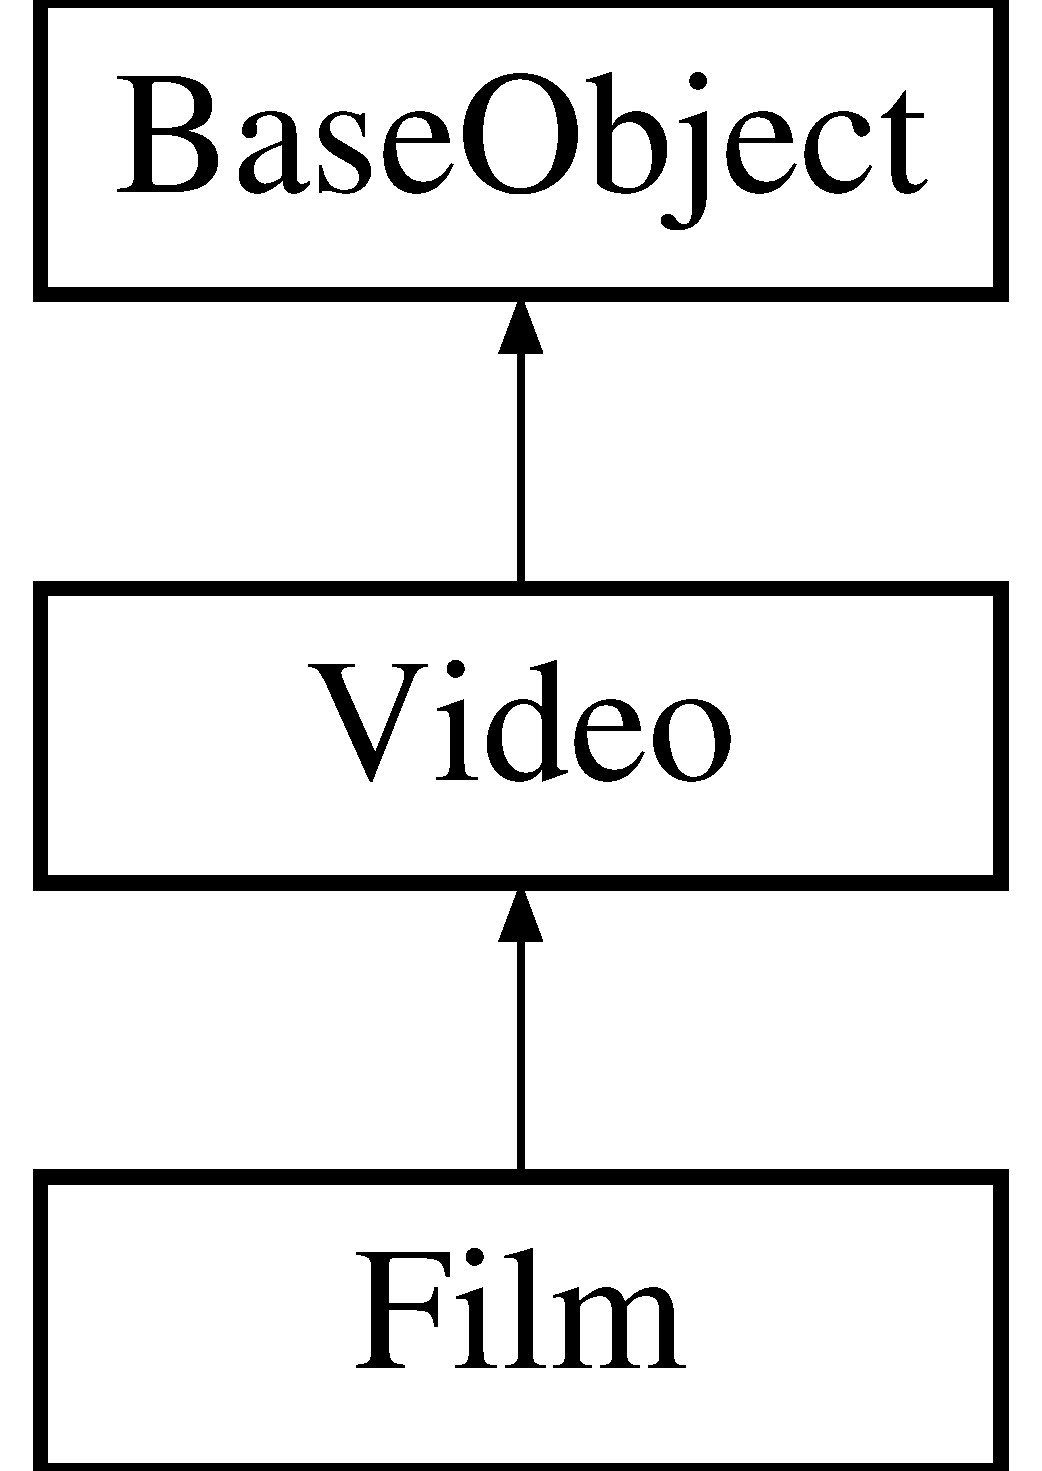
\includegraphics[height=2.000000cm]{classVideo}
\end{center}
\end{figure}
\subsection*{Public Member Functions}
\begin{DoxyCompactItemize}
\item 
\hypertarget{classVideo_ad0277d8e5772008e22ac2948e03e103b}{\hyperlink{classVideo_ad0277d8e5772008e22ac2948e03e103b}{Video} (std\-::string name=\char`\"{}new video\char`\"{}, time\-\_\-t creat=time(N\-U\-L\-L), std\-::string path=\char`\"{}$\sim$/new\-\_\-video\char`\"{}, int duration=0)}\label{classVideo_ad0277d8e5772008e22ac2948e03e103b}

\begin{DoxyCompactList}\small\item\em Parametered Constructor. \end{DoxyCompactList}\item 
\hyperlink{classVideo_aebf7e2a8fa2bbd79335b1cf35925d190}{$\sim$\-Video} ()
\begin{DoxyCompactList}\small\item\em Parameterless Destructor. \end{DoxyCompactList}\item 
\hypertarget{classVideo_ad947c70ddc192dcb8e511fda6a616a4f}{virtual std\-::string \hyperlink{classVideo_ad947c70ddc192dcb8e511fda6a616a4f}{to\-String} () const }\label{classVideo_ad947c70ddc192dcb8e511fda6a616a4f}

\begin{DoxyCompactList}\small\item\em Returns multi-\/line string containing formatted description of object. \end{DoxyCompactList}\end{DoxyCompactItemize}


\subsection{Detailed Description}
\hyperlink{classVideo}{Video} file object. 

This class describes a \hyperlink{classVideo}{Video} object 

\subsection{Constructor \& Destructor Documentation}
\hypertarget{classVideo_aebf7e2a8fa2bbd79335b1cf35925d190}{\index{Video@{Video}!$\sim$\-Video@{$\sim$\-Video}}
\index{$\sim$\-Video@{$\sim$\-Video}!Video@{Video}}
\subsubsection[{$\sim$\-Video}]{\setlength{\rightskip}{0pt plus 5cm}Video\-::$\sim$\-Video (
\begin{DoxyParamCaption}
{}
\end{DoxyParamCaption}
)}}\label{classVideo_aebf7e2a8fa2bbd79335b1cf35925d190}


Parameterless Destructor. 

Implemetation is empty as there is nothing to delete. 

The documentation for this class was generated from the following files\-:\begin{DoxyCompactItemize}
\item 
Video.\-h\item 
Video.\-cpp\end{DoxyCompactItemize}

%--- End generated contents ---

% Index
\newpage
\phantomsection
\addcontentsline{toc}{chapter}{Index}
\printindex

\end{document}
